
%%%  تالار گفتگوی پارسی‌لاتک،       http://forum.parsilatex.com


%        روش اجرا.: 2 بار F1 ، 2 بار  F11(به منظور تولید مراجع) ، دوبار Ctrl+Alt+I (به منظور تولید نمایه) و دو بار F1 -------> مشاهده Pdf
%%%%%%%%%%%%%%%%%%%%%%%%%%%%%%%%%%%%%%%%%%%%%%%%%%%%%%
%   TeXstudio as your IDE
%%  برای compile در TeXstudio تنها کافی است منوی Options->Configure TeXstudio را زده و در پنجره Configure TeXstudio در بخش Build گزینه Default Compiler را به XeLaTeX تغییر دهید. سند شما به راحتی compile خواهد شد.
%   F1 & F5 : Build & view
%   F6      : Compile
%   F7      : View
%   --------------
%%%%%%%%%%%%%%%%%%%%%%%%%%%%%%%%%%%%%%%%%%%%%%%%%%%%%%
%%% !TEX TS-program = XeLaTeX
\documentclass[oneside,msc,12pt]{main}
\usepackage{ragged2e}
\newcommand\pd[2]{\displaystyle\frac{\partial #1}{\partial #2}}

\usepackage[acronym]{glossaries}
\usepackage{calc}
%\usepackage{caption_2010-01-09}
\usepackage{array}
\usepackage{makecell}
\usepackage{multirow}
\usepackage{longtable}
%\usepackage{graphicx}
%\usepackage{array}
\usepackage{rotating}

\usepackage{lscape}
\usepackage{pdflscape}
\usepackage{wasysym}
%\usepackage{arabicore}
%\usepackage{caption_2019-09-01}
\makeglossary
\newacronym{co}{CO}{heavy-industrit-sd}
%\usepackage{bit}
%\usepackage{natbib}
%\addbibresource{references.bib}
\usepackage{forest}
\usepackage{fontspec}

\usepackage{tikz}
\usetikzlibrary{shapes,arrows,trees,calc}
% در این فایل، دستورها و تنظیمات مورد نیاز، آورده شده است.
%-------------------------------------------------------------------------------------------------------------------
% در ورژن جدید زی‌پرشین برای تایپ متن‌های ریاضی، این سه بسته، حتماً باید فراخوانی شود.
\usepackage{amsthm,amssymb,amsmath,amsfonts}
% بسته‌ای برای تنطیم حاشیه‌های بالا، پایین، چپ و راست صفحه
\usepackage[top=30mm, bottom=30mm, left=25mm, right=30mm]{geometry}
% بسته‌‌ای برای ظاهر شدن شکل‌ها و تصاویر متن
\usepackage{graphicx}
\usepackage{color}
%بسته‌ای برای تنظیم فاصله عمودی خط‌های متن
\usepackage{setspace}
\usepackage{titletoc}
\usepackage{tocloft}
%با فعال کردن بسته زیر فوت‌نوت‌ها در هر صفحه ریست می‌شوند. حالت پیش‌فرض آن ریست شدن در هر فصل می‌باشد.
%\usepackage[perpage]{footmisc}
\usepackage{enumitem}
%\usepackage{titlesec}
% بسته‌ و دستوراتی برای ایجاد لینک‌های رنگی با امکان جهش
\usepackage[pagebackref=false,colorlinks,linkcolor=blue,citecolor=red]{hyperref}
\usepackage[nameinlink]{cleveref}%capitalize,,noabbrev
 \AtBeginDocument{%
    \crefname{equation}{برابری}{equations}%
    \crefname{chapter}{فصل}{chapters}%
    \crefname{section}{بخش}{sections}%
    \crefname{appendix}{پیوست}{appendices}%
    \crefname{enumi}{مورد}{items}%
    \crefname{footnote}{زیرنویس}{footnotes}%
    \crefname{figure}{شکل}{figures}%
    \crefname{table}{جدول}{tables}%
    \crefname{theorem}{قضیه}{theorems}%
    \crefname{lemma}{لم}{lemmas}%
    \crefname{corollary}{نتیجه}{corollaries}%
    \crefname{proposition}{گزاره}{propositions}%
    \crefname{definition}{تعریف}{definitions}%
    \crefname{result}{نتیجه}{results}%
    \crefname{example}{مثال}{examples}%
    \crefname{remark}{نکته}{remarks}%
    \crefname{note}{یادداشت}{notes}%
}
% چنانچه قصد پرینت گرفتن نوشته خود را دارید، خط بالا را غیرفعال و  از دستور زیر استفاده کنید چون در صورت استفاده از دستور زیر‌‌، 
% لینک‌ها به رنگ سیاه ظاهر خواهند شد که برای پرینت گرفتن، مناسب‌تر است
%\usepackage[pagebackref=false]{hyperref}
% بسته‌ لازم برای تنظیم سربرگ‌ها
\usepackage{fancyhdr}
% بسته‌ای برای ظاهر شدن «مراجع»  در فهرست مطالب
\usepackage[nottoc]{tocbibind}
% دستورات مربوط به ایجاد نمایه
\usepackage{makeidx,multicol}
\setlength{\columnsep}{1.5cm}

%%%%%%%%%%%%%%%%%%%%%%%%%%
\usepackage{verbatim}
\makeindex
\usepackage{sectsty}
% فراخوانی بسته زی‌پرشین و تعریف قلم فارسی و انگلیسی
\usepackage{xepersian}%[extrafootnotefeatures]
\SepMark{-}
%حتماً از تک لایو 2014 استفاده کنید.\settextfont [Scale = 1.1] {bnazanin.ttf}
%\setdigitfont [Scale = 1.1] {Times New Roman.ttf}
\setdigitfont [Scale = 1.1,BoldFont={BNaznnBd.ttf}] {X Nazanin.ttf}
\setlatintextfont [Scale = 1.05] {Times New Roman.ttf}
\settextfont[Scale=1.2,%
BoldFont={BNaznnBd.ttf},%\textbf{}
%BoldFeatures={FakeBold=1.2},%
%BoldFont={X Nazanin Bold.ttf},%
ItalicFont={bnazanin.ttf},%
ItalicFeatures={FakeSlant=.3},%
BoldItalicFont={bnazanin.ttf},%
BoldItalicFeatures={FakeSlant=.3,FakeBold=1}%
]{bnazanin.ttf}
\renewcommand{\labelitemi}{$\bullet$}
%%%%%%%%%%%%%%%%%%%%%%%%%%
% چنانچه می‌خواهید اعداد در فرمول‌ها، انگلیسی باشد، خط زیر را غیرفعال کنید.
%در غیر اینصورت حتماً فونت PGaramond را نصب کنید.
%\setdigitfont[Scale=1.1]{PGaramond}%%Yas
%%%%%%%%%%%%%%%%%%%%%%%%%%
% تعریف قلم‌های فارسی اضافی برای استفاده در بعضی از قسمت‌های متن
\defpersianfont\nastaliq[Scale=2]{IranNastaliq.ttf}
\defpersianfont\chapternumber[Scale=3]{BNaznnBd.ttf}
%\chapterfont{\centering}%
%%%%%%%%%%%%%%%%%%%%%%%%%%
% دستوری برای تغییر نام کلمه «اثبات» به «برهان»
\renewcommand\proofname{\textbf{برهان}}

% دستوری برای تغییر نام کلمه «کتاب‌نامه» به «منابع و مراجع«
\renewcommand{\bibname}{منابع و مراجع}


% Headings for every page of ToC, LoF and Lot
\setlength{\cftbeforetoctitleskip}{-1.2em}
\setlength{\cftbeforelottitleskip}{-1.2em}
\setlength{\cftbeforeloftitleskip}{-1.2em}
\setlength{\cftaftertoctitleskip}{-1em}
\setlength{\cftafterlottitleskip}{-1em}
\setlength{\cftafterloftitleskip}{-1em}
%%\makeatletter
%%%%\renewcommand{\l@chapter}{\@dottedtocline{1}{1em\bfseries}{1em}}
%%%%\renewcommand{\l@section}{\@dottedtocline{2}{2em}{2em}}
%%%%\renewcommand{\l@subsection}{\@dottedtocline{3}{3em}{3em}}
%%%%\renewcommand{\l@subsubsection}{\@dottedtocline{4}{4em}{4em}}
%%%%\makeatother


\newcommand\tocheading{\par عنوان\hfill صفحه \par}
\newcommand\lofheading{\hspace*{.5cm}\figurename\hfill صفحه \par}
\newcommand\lotheading{\hspace*{.5cm}\tablename\hfill صفحه \par}

\renewcommand{\cftchapleader}{\cftdotfill{\cftdotsep}}
\renewcommand{\cfttoctitlefont}{\hspace*{\fill}\LARGE\bfseries}%\Large
\renewcommand{\cftaftertoctitle}{\hspace*{\fill}}
\renewcommand{\cftlottitlefont}{\hspace*{\fill}\LARGE\bfseries}%\Large
\renewcommand{\cftafterlottitle}{\hspace*{\fill}}
\renewcommand{\cftloftitlefont}{\hspace*{\fill}\LARGE\bfseries}
\renewcommand{\cftafterloftitle}{\hspace*{\fill}}

%%%%%%%%%%%%%%%%%%%%%%%%%%
% تعریف و نحوه ظاهر شدن عنوان قضیه‌ها، تعریف‌ها، مثال‌ها و ...
%برای شماره گذاری سه تایی قضیه ها
\theoremstyle{definition}
\newtheorem{definition}{تعریف}[section]
\newtheorem{remark}[definition]{نکته}
\newtheorem{note}[definition]{یادداشت}
\newtheorem{example}[definition]{نمونه}
\newtheorem{question}[definition]{سوال}
\newtheorem{remember}[definition]{یاداوری}
\theoremstyle{theorem}
\newtheorem{theorem}[definition]{قضیه}
\newtheorem{lemma}[definition]{لم}
\newtheorem{proposition}[definition]{گزاره}
\newtheorem{corollary}[definition]{نتیجه}
%%%%%%%%%%%%%%%%%%%%%%%%
%%%%%%%%%%%%%%%%%%%
%%% برای شماره گذاری چهارتایی قضیه ها و ...
%%\newtheorem{definition1}[subsubsection]{تعریف}
%%\newtheorem{theorem1}[subsubsection]{قضیه}
%%\newtheorem{lemma1}[subsubsection]{لم}
%%\newtheorem{proposition1}[subsubsection]{گزاره}
%%\newtheorem{corollary1}[subsubsection]{نتیجه}
%%\newtheorem{remark1}[subsubsection]{نکته}
%%\newtheorem{example1}[subsubsection]{مثال}
%%\newtheorem{question1}[subsubsection]{سوال}

%%%%%%%%%%%%%%%%%%%%%%%%%%%%

% دستورهایی برای سفارشی کردن صفحات اول فصل‌ها
\makeatletter
\newcommand\mycustomraggedright{%
 \if@RTL\raggedleft%
 \else\raggedright%
 \fi}
\def\@makechapterhead#1{%
\thispagestyle{style1}
\vspace*{20\p@}%
{\parindent \z@ \mycustomraggedright
\ifnum \c@secnumdepth >\m@ne
\if@mainmatter

\bfseries{\Huge \@chapapp}\small\space {\chapternumber\thechapter}
\par\nobreak
\vskip 0\p@
\fi
\fi
\interlinepenalty\@M 
\Huge \bfseries #1\par\nobreak
\vskip 120\p@

}

%\thispagestyle{empty}
\newpage}
\bidi@patchcmd{\@makechapterhead}{\thechapter}{\tartibi{chapter}}{}{}
\bidi@patchcmd{\chaptermark}{\thechapter}{\tartibi{chapter}}{}{}
\makeatother

\pagestyle{fancy}
\renewcommand{\chaptermark}[1]{\markboth{\chaptername~\tartibi{chapter}: #1}{}}

\fancypagestyle{style1}{
\fancyhf{} 
\fancyfoot[c]{\thepage}
\fancyhead[R]{\leftmark}%
\renewcommand{\headrulewidth}{1.2pt}
}


\fancypagestyle{style2}{
\fancyhf{}
\fancyhead[R]{چکیده}
\fancyfoot[C]{\thepage{}}
\renewcommand{\headrulewidth}{1.2pt}
}

\fancypagestyle{style3}{%
  \fancyhf{}%
  \fancyhead[R]{فهرست نمادها}
  \fancyfoot[C]{\thepage}%
  \renewcommand{\headrulewidth}{1.2pt}%
}

\fancypagestyle{style4}{%
  \fancyhf{}%
  \fancyhead[R]{فهرست جداول}
  \fancyfoot[C]{\thepage}%
  \renewcommand{\headrulewidth}{1.2pt}%
}

\fancypagestyle{style5}{%
  \fancyhf{}%
  \fancyhead[R]{فهرست اشکال}
  \fancyfoot[C]{\thepage}%
  \renewcommand{\headrulewidth}{1.2pt}%
}

\fancypagestyle{style6}{%
  \fancyhf{}%
  \fancyhead[R]{فهرست مطالب}
  \fancyfoot[C]{\thepage}%
  \renewcommand{\headrulewidth}{1.2pt}%
}

\fancypagestyle{style7}{%
  \fancyhf{}%
  \fancyhead[R]{نمایه}
  \fancyfoot[C]{\thepage}%
  \renewcommand{\headrulewidth}{1.2pt}%
}

\fancypagestyle{style8}{%
  \fancyhf{}%
  \fancyhead[R]{منابع و مراجع}
  \fancyfoot[C]{\thepage}%
  \renewcommand{\headrulewidth}{1.2pt}%
}
\fancypagestyle{style9}{%
  \fancyhf{}%
  \fancyhead[R]{واژه‌نامه‌ی فارسی به انگلیسی}
  \fancyfoot[C]{\thepage}%
  \renewcommand{\headrulewidth}{1.2pt}%
}
%


%دستور حذف نام لیست تصاویر و لیست جداول از فهرست مطالب
\newcommand*{\BeginNoToc}{%
  \addtocontents{toc}{%
    \edef\protect\SavedTocDepth{\protect\the\protect\value{tocdepth}}%
  }%
  \addtocontents{toc}{%
    \protect\setcounter{tocdepth}{-10}%
  }%
}
\newcommand*{\EndNoToc}{%
  \addtocontents{toc}{%
    \protect\setcounter{tocdepth}{\protect\SavedTocDepth}%
  }%
}
\newcounter{savepage}
\renewcommand{\listfigurename}{فهرست اشکال}
\renewcommand{\listtablename}{فهرست جداول}
%\renewcommand\cftsecleader{\cftdotfill{\cftdotsep}}
%%%%%%%%%%%%%%%%%%%%%%%%%%%%%
%%%%%%%%%%%%%%%%%%%%%%%%%%%%
% for numbering subsubsections
\setcounter{secnumdepth}{3}
%to include subsubsections in the table of contents
\setcounter{tocdepth}{3}

\begin{document}
\baselineskip=.75cm
\linespread{1.75}
%% -!TEX root = AUTthesis.tex
% در این فایل، عنوان پایان‌نامه، مشخصات خود، متن تقدیمی‌، ستایش، سپاس‌گزاری و چکیده پایان‌نامه را به فارسی، وارد کنید.
% توجه داشته باشید که جدول حاوی مشخصات پروژه/پایان‌نامه/رساله و همچنین، مشخصات داخل آن، به طور خودکار، درج می‌شود.
%%%%%%%%%%%%%%%%%%%%%%%%%%%%%%%%%%%%
% دانشکده، آموزشکده و یا پژوهشکده  خود را وارد کنید
\faculty{دانشکده ...}
% گرایش و گروه آموزشی خود را وارد کنید
\department{گرایش ...}
% عنوان پایان‌نامه را وارد کنید
\fatitle{عنوان پایان نامه-دستورالعمل و راهنمای نگارش
\\[.75 cm]
 پایان‌نامه}
% نام استاد(ان) راهنما را وارد کنید
\firstsupervisor{نام کامل استاد راهنما}
%\secondsupervisor{استاد راهنمای دوم}
% نام استاد(دان) مشاور را وارد کنید. چنانچه استاد مشاور ندارید، دستور پایین را غیرفعال کنید.
\firstadvisor{نام کامل استاد مشاور}
%\secondadvisor{استاد مشاور دوم}
% نام نویسنده را وارد کنید
\name{نام }
% نام خانوادگی نویسنده را وارد کنید
\surname{و نام خانوادگی کامل نویسنده}
%%%%%%%%%%%%%%%%%%%%%%%%%%%%%%%%%%
\thesisdate{ماه و سال}

% چکیده پایان‌نامه را وارد کنید
\fa-abstract{
در اين قسمت چكيده پایان نامه نوشته مي‌شو‌د‌.‌ چكيده بايد جامع و بيان‌كننده‌ خلاصه‌اي از اقدامات انجام‌شده باشد. در چكيده باید از ارجاع به مرجع و ذكر روابط رياضي، بيان تاريخچه و تعريف مسئله خودداري ‌شود. 
}


% کلمات کلیدی پایان‌نامه را وارد کنید
\keywords{کلیدواژه اول، ...، کلیدواژه پنجم (نوشتن سه تا پنج واژه کلیدی ضروری است)}



\ICStitle
%%%%%%%%%%%%%%%%%%%%%%%%%%%%%%%%%%
\vspace*{7cm}
\thispagestyle{empty}
\begin{center}

\includegraphics[height=5cm,width=12cm]{besm}
\end{center}
% دستور زیر برای شماره گذاری صفحات قبل از فصل اول با حروف ابجد است.
\pagenumbering{alph}
%-----------------------------------------------------------------------------
% فایل زیر دستورات مربوط به نمایش صفحات فهرست مطالب- فهرست اشکال و جداول است.
%{\pagestyle{style2}
%\tableofcontents}\newpage
%
%\listoffigures
\cleardoublepage
\pagestyle{style6}
\tableofcontents
\pagestyle{style6}
\cleardoublepage
%اگر لیست تصاویر و لیست جداول ندارید ، کدهای زیر را با گذاشتن % در ابتدای آنها، غیرفعال کنید.
\BeginNoToc
%============
\addtocontents{lof}{\lofheading}% add heading to the first page in LoF
\pagestyle{style5}
\listoffigures
\thispagestyle{style5}
\cleardoublepage
%============
\addtocontents{lot}{\lotheading}% add heading to the first page in LoT
\thispagestyle{style4}
\listoftables
\thispagestyle{style4}
%============
%\cleardoublepage
%
\cleardoublepage
\setcounter{savepage}{\arabic{page}}
\mainmatter
\addtocontents{toc}{\tocheading}% add heading to the first page in ToC, after frontmatter entries
\EndNoToc
%-------------------------------------------------------------------------symbols(فهرست نمادها)
%%%%%%%%%%%%%

{\centering\LARGE\textbf{فهرست نمادها}\par}%

\pagenumbering{alph}
\setcounter{page}{\thesavepage}
%\setcounter{page}{6}
\vspace*{1cm}

\pagestyle{style3}
%\thispagestyle{empty}
%\addcontentsline{toc}{chapter}{فهرست نمادها}
\symb{\text{ نماد}}{مفهوم}
\\
%مقادیر بالا را تغییر ندهید
%%%%%%%%%%%%%%%%%%%%%%%%%%%%%%%%%%%%%%%%%%%%%%%%%%%%%%%%%
\symb{\mathbb{R}^n}{
فضای اقلیدسی با بعد $n$
}
\symb{\mathbb{S}^n}{
کره یکه $n$ بعدی
}
\symb{M^m}{
خمینه $m$-بعدی $M$
}
\symb{\mathfrak{X}(M)}{
جبر میدان‌های  برداری هموار روی $M$
}
\symb{\mathfrak{X}^1(M)}{
مجموعه میدان‌های برداری هموار یکه روی $(M,g)$ 
}
\symb{\Omega^p(M)}{
مجموعه $p$-فرمی‌های روی خمینه $M$
}
\symb{Q}{
اپراتور ریچی
}
\symb{\mathcal{R}}{
تانسور انحنای ریمان
}
\symb{ric}{
تانسور ریچی
}
\symb{L}{
مشتق لی
}
\symb{\Phi}{
2-فرم اساسی خمینه تماسی
}
\symb{\nabla}{
التصاق لوی-چویتای
}
\symb{\Delta}{
لاپلاسین ناهموار
}
\symb{\nabla^*}{
عملگر خودالحاق صوری القا شده از التصاق لوی-چویتای
}
\symb{g_s}{
متر ساساکی
}
\symb{\nabla}{
التصاق لوی-چویتای وابسته به متر ساساکی
}
\symb{\Delta}{
عملگر لاپلاس-بلترامی روی $p$-فرم‌ها
}

%%%%%%%%%%%%%%%%%%%%%%%%%%%%%%%%%%%%%%%

\thispagestyle{style3}
\newpage
%\pagestyle{style1}
%%%%%%%%%%%%%%%%%%%%%%%%%%%%%%%%%%%%


\pagenumbering{arabic}
\pagestyle{style1}
%--------------------------------------------------------------------------chapters(فصل ها)
\chapter{راهنمای استفاده از الگوی لاتک دانشگاه صنعتی امیرکبیر(پلی‌تکنیک تهران)}

\section{مقدمه}
حروف‌چینی پروژه کارشناسی، پایان‌نامه یا رساله یکی از موارد پرکاربرد استفاده از زی‌پرشین است. از طرفی، یک پروژه، پایان‌نامه یا رساله،  احتیاج به تنظیمات زیادی از نظر صفحه‌آرایی  دارد که ممکن است برای
یک کاربر مبتدی، مشکل باشد. به همین خاطر، برای راحتی کار کاربر، یک کلاس با نام 
\verb;AUTthesis;
 برای حروف‌چینی پروژه‌ها، پایان‌نامه‌ها و رساله‌های دانشگاه صنعتی امیرکبیر با استفاده از نرم‌افزار زی‌پرشین،  آماده شده است. این فایل به 
گونه‌ای طراحی شده است که کلیه خواسته‌های مورد نیاز  مدیریت تحصیلات تکمیلی دانشگاه صنعتی امیرکبیر را برآورده می‌کند و نیز، حروف‌چینی بسیاری
از قسمت‌های آن، به طور خودکار انجام می‌شود.

کلیه فایل‌های لازم برای حروف‌چینی با کلاس گفته شده، داخل پوشه‌ای به نام
\verb;AUTthesis;
  قرار داده شده است. توجه داشته باشید که برای استفاده از این کلاس باید فونت‌های
  \verb;Nazanin B;،
 \verb;PGaramond;
 و
  \verb;IranNastaliq;
    روی سیستم شما نصب شده باشد.
\section{این همه فایل؟!}\label{sec2}
از آنجایی که یک پایان‌نامه یا رساله، یک نوشته بلند محسوب می‌شود، لذا اگر همه تنظیمات و مطالب پایان‌نامه را داخل یک فایل قرار بدهیم، باعث شلوغی
و سردرگمی می‌شود. به همین خاطر، قسمت‌های مختلف پایان‌نامه یا رساله  داخل فایل‌های جداگانه قرار گرفته است. مثلاً تنظیمات پایه‌ای کلاس، داخل فایل
\verb;AUTthesis.cls;، 
تنظیمات قابل تغییر توسط کاربر، داخل 
\verb;commands.tex;،
قسمت مشخصات فارسی پایان‌نامه، داخل 
\verb;fa_title.tex;,
مطالب فصل اول، داخل 
\verb;chapter1;
و ... قرار داده شده است. نکته مهمی که در اینجا وجود دارد این است که از بین این  فایل‌ها، فقط فایل 
\verb;AUTthesis.tex;
قابل اجرا است. یعنی بعد از تغییر فایل‌های دیگر، برای دیدن نتیجه تغییرات، باید این فایل را اجرا کرد. بقیه فایل‌ها به این فایل، کمک می‌کنند تا بتوانیم خروجی کار را ببینیم. اگر به فایل 
\verb;AUTthesis.tex;
دقت کنید، متوجه می‌شوید که قسمت‌های مختلف پایان‌نامه، توسط دستورهایی مانند 
\verb;input;
و
\verb;include;
به فایل اصلی، یعنی 
\verb;AUTthesis.tex;
معرفی شده‌اند. بنابراین، فایلی که همیشه با آن سروکار داریم، فایل 
\verb;AUTthesis.tex;
است.
در این فایل، فرض شده است که پایان‌نامه یا رساله شما، از5 فصل و یک پیوست، تشکیل شده است. با این حال، اگر
  پایان‌نامه یا رساله شما، بیشتر از 5 فصل و یک پیوست است، باید خودتان فصل‌های بیشتر را به این فایل، اضافه کنید. این کار، بسیار ساده است. فرض کنید بخواهید یک فصل دیگر هم به پایان‌نامه، اضافه کنید. برای این کار، کافی است یک فایل با نام 
\verb;chapter6;
و با پسوند 
\verb;.tex;
بسازید و آن را داخل پوشه 
\verb;AUTthesis;
قرار دهید و سپس این فایل را با دستور 
\texttt{\textbackslash include\{chapter6\}}
داخل فایل
\verb;AUTthesis.tex;
و بعد از دستور
\texttt{\textbackslash include\{chapter6\}}
 قرار دهید.

\section{از کجا شروع کنم؟}
قبل از هر چیز، بدیهی است که باید یک توزیع تِک مناسب مانند 
\verb;Live TeX;
و یک ویرایش‌گر تِک مانند
\verb;Texmaker;
را روی سیستم خود نصب کنید.  نسخه بهینه شده 
\verb;Texmaker;
را می‌توانید  از سایت 
 \href{http://www.parsilatex.com}{پارسی‌لاتک}%
\LTRfootnote{\url{http://www.parsilatex.com}}
 و
\verb;Live TeX;
را هم می‌توانید از 
 \href{http://www.tug.org/texlive}{سایت رسمی آن}%
\LTRfootnote{\url{http://www.tug.org/texlive}}
 دانلود کنید.
 
در مرحله بعد، سعی کنید که  یک پشتیبان از پوشه 
\verb;AUTthesis;
 بگیرید و آن را در یک جایی از هارددیسک سیستم خود ذخیره کنید تا در صورت خراب کردن فایل‌هایی که در حال حاضر، با آن‌ها کار می‌کنید، همه چیز را از 
 دست ندهید.
 
 حال اگر نوشتن پایان‌نامه اولین تجربه شما از کار با لاتک است، توصیه می‌شود که یک‌بار به طور سرسری، کتاب «%
\href{http://www.tug.ctan.org/tex-archive/info/lshort/persian/lshort.pdf}{مقدمه‌ای نه چندان کوتاه بر
\lr{\LaTeXe}}\LTRfootnote{\url{http://www.tug.ctan.org/tex-archive/info/lshort/persian/lshort.pdf}}»
   ترجمه دکتر مهدی امیدعلی، عضو هیات علمی دانشگاه شاهد را مطالعه کنید. این کتاب، کتاب بسیار کاملی است که خیلی از نیازهای شما در ارتباط با حروف‌چینی را برطرف می‌کند.
 
 
بعد از موارد گفته شده، فایل 
\verb;AUTthesis.tex;
و
\verb;fa_title;
را باز کنید و مشخصات پایان‌نامه خود مثل نام، نام خانوادگی، عنوان پایان‌نامه و ... را جایگزین مشخصات موجود در فایل
\verb;fa_title;
 کنید. دقت داشته باشید که نیازی نیست 
نگران چینش این مشخصات در فایل پی‌دی‌اف خروجی باشید. فایل 
\verb;AUTthesis.cls;
همه این کارها را به طور خودکار برای شما انجام می‌دهد. در ضمن، موقع تغییر دادن دستورهای داخل فایل
\verb;fa_title;
 کاملاً دقت کنید. این دستورها، خیلی حساس هستند و ممکن است با یک تغییر کوچک، موقع اجرا، خطا بگیرید. برای دیدن خروجی کار، فایل 
\verb;fa_title;
 را 
\verb;Save;، 
(نه 
\verb;As Save;)
کنید و بعد به فایل 
\verb;AUTthesis.tex;
برگشته و آن را اجرا کنید. حال اگر می‌خواهید مشخصات انگلیسی پایان‌نامه را هم عوض کنید، فایل 
\verb;en_title;
را باز کنید و مشخصات داخل آن را تغییر دهید.%
\RTLfootnote{
برای نوشتن پروژه کارشناسی، نیازی به وارد کردن مشخصات انگلیسی پروژه نیست. بنابراین، این مشخصات، به طور خودکار،
نادیده گرفته می‌شود.
}
 در اینجا هم برای دیدن خروجی، باید این فایل را 
\verb;Save;
کرده و بعد به فایل 
\verb;AUTthesis.tex;
برگشته و آن را اجرا کرد.

برای راحتی بیشتر، 
فایل 
\verb;AUTthesis.cls;
طوری طراحی شده است که کافی است فقط  یک‌بار مشخصات پایان‌نامه  را وارد کنید. هر جای دیگر که لازم به درج این مشخصات باشد، این مشخصات به طور خودکار درج می‌شود. با این حال، اگر مایل بودید، می‌توانید تنظیمات موجود را تغییر دهید. توجه داشته باشید که اگر کاربر مبتدی هستید و یا با ساختار فایل‌های  
\verb;cls;
 آشنایی ندارید، به هیچ وجه به این فایل، یعنی فایل 
\verb;AUTthesis.cls;
دست نزنید.

نکته دیگری که باید به آن توجه کنید این است که در فایل 
\verb;AUTthesis.cls;،
سه گزینه به نام‌های
\verb;bsc;,
\verb;msc;
و
\verb;phd;
برای تایپ پروژه، پایان‌نامه و رساله،
طراحی شده است. بنابراین اگر قصد تایپ پروژه کارشناسی، پایان‌نامه یا رساله را دارید، 
 در فایل 
\verb;AUTthesis.tex;
باید به ترتیب از گزینه‌های
\verb;bsc;،
\verb;msc;
و
\verb;phd;
استفاده کنید. با انتخاب هر کدام از این گزینه‌ها، تنظیمات مربوط به آنها به طور خودکار، اعمل می‌شود.

\section{مطالب پایان‌نامه را چطور بنویسم؟}
\subsection{نوشتن فصل‌ها}
همان‌طور که در بخش 
\ref{sec2}
گفته شد، برای جلوگیری از شلوغی و سردرگمی کاربر در هنگام حروف‌چینی، قسمت‌های مختلف پایان‌نامه از جمله فصل‌ها، در فایل‌های جداگانه‌ای قرار داده شده‌اند. 
بنابراین، اگر می‌خواهید مثلاً مطالب فصل ۱ را تایپ کنید، باید فایل‌های 
\verb;AUTthesis.tex;
و
\verb;chapter1;
را باز کنید و محتویات داخل فایل 
\verb;chapter1;
را پاک کرده و مطالب خود را تایپ کنید. توجه کنید که همان‌طور که قبلاً هم گفته شد، تنها فایل قابل اجرا، فایل 
\verb;AUTthesis.tex;
است. لذا برای دیدن حاصل (خروجی) فایل خود، باید فایل  
\verb;chapter1;
را 
\verb;Save;
کرده و سپس فایل 
\verb;AUTthesis.tex;
را اجرا کنید. یک نکته بدیهی که در اینجا وجود دارد، این است که لازم نیست که فصل‌های پایان‌نامه را به ترتیب تایپ کنید. می‌توانید ابتدا مطالب فصل ۳ را تایپ کنید و سپس مطالب فصل ۱ را تایپ کنید.

نکته بسیار مهمی که در اینجا باید گفته شود این است که سیستم
\lr{\TeX},
محتویات یک فایل تِک را به ترتیب پردازش می‌کند. به عنوان مثال، اگه فایلی، دارای ۴ خط دستور باشد، ابتدا خط ۱، بعد خط ۲، بعد خط ۳ و در آخر، خط ۴ پردازش می‌شود. بنابراین، اگر مثلاً مشغول تایپ مطالب فصل ۳ هستید، بهتر است
که دو دستور
\verb~\chapter{راهنمای استفاده از الگوی لاتک دانشگاه صنعتی امیرکبیر(پلی‌تکنیک تهران)}

\section{مقدمه}
حروف‌چینی پروژه کارشناسی، پایان‌نامه یا رساله یکی از موارد پرکاربرد استفاده از زی‌پرشین است. از طرفی، یک پروژه، پایان‌نامه یا رساله،  احتیاج به تنظیمات زیادی از نظر صفحه‌آرایی  دارد که ممکن است برای
یک کاربر مبتدی، مشکل باشد. به همین خاطر، برای راحتی کار کاربر، یک کلاس با نام 
\verb;AUTthesis;
 برای حروف‌چینی پروژه‌ها، پایان‌نامه‌ها و رساله‌های دانشگاه صنعتی امیرکبیر با استفاده از نرم‌افزار زی‌پرشین،  آماده شده است. این فایل به 
گونه‌ای طراحی شده است که کلیه خواسته‌های مورد نیاز  مدیریت تحصیلات تکمیلی دانشگاه صنعتی امیرکبیر را برآورده می‌کند و نیز، حروف‌چینی بسیاری
از قسمت‌های آن، به طور خودکار انجام می‌شود.

کلیه فایل‌های لازم برای حروف‌چینی با کلاس گفته شده، داخل پوشه‌ای به نام
\verb;AUTthesis;
  قرار داده شده است. توجه داشته باشید که برای استفاده از این کلاس باید فونت‌های
  \verb;Nazanin B;،
 \verb;PGaramond;
 و
  \verb;IranNastaliq;
    روی سیستم شما نصب شده باشد.
\section{این همه فایل؟!}\label{sec2}
از آنجایی که یک پایان‌نامه یا رساله، یک نوشته بلند محسوب می‌شود، لذا اگر همه تنظیمات و مطالب پایان‌نامه را داخل یک فایل قرار بدهیم، باعث شلوغی
و سردرگمی می‌شود. به همین خاطر، قسمت‌های مختلف پایان‌نامه یا رساله  داخل فایل‌های جداگانه قرار گرفته است. مثلاً تنظیمات پایه‌ای کلاس، داخل فایل
\verb;AUTthesis.cls;، 
تنظیمات قابل تغییر توسط کاربر، داخل 
\verb;commands.tex;،
قسمت مشخصات فارسی پایان‌نامه، داخل 
\verb;fa_title.tex;,
مطالب فصل اول، داخل 
\verb;chapter1;
و ... قرار داده شده است. نکته مهمی که در اینجا وجود دارد این است که از بین این  فایل‌ها، فقط فایل 
\verb;AUTthesis.tex;
قابل اجرا است. یعنی بعد از تغییر فایل‌های دیگر، برای دیدن نتیجه تغییرات، باید این فایل را اجرا کرد. بقیه فایل‌ها به این فایل، کمک می‌کنند تا بتوانیم خروجی کار را ببینیم. اگر به فایل 
\verb;AUTthesis.tex;
دقت کنید، متوجه می‌شوید که قسمت‌های مختلف پایان‌نامه، توسط دستورهایی مانند 
\verb;input;
و
\verb;include;
به فایل اصلی، یعنی 
\verb;AUTthesis.tex;
معرفی شده‌اند. بنابراین، فایلی که همیشه با آن سروکار داریم، فایل 
\verb;AUTthesis.tex;
است.
در این فایل، فرض شده است که پایان‌نامه یا رساله شما، از5 فصل و یک پیوست، تشکیل شده است. با این حال، اگر
  پایان‌نامه یا رساله شما، بیشتر از 5 فصل و یک پیوست است، باید خودتان فصل‌های بیشتر را به این فایل، اضافه کنید. این کار، بسیار ساده است. فرض کنید بخواهید یک فصل دیگر هم به پایان‌نامه، اضافه کنید. برای این کار، کافی است یک فایل با نام 
\verb;chapter6;
و با پسوند 
\verb;.tex;
بسازید و آن را داخل پوشه 
\verb;AUTthesis;
قرار دهید و سپس این فایل را با دستور 
\texttt{\textbackslash include\{chapter6\}}
داخل فایل
\verb;AUTthesis.tex;
و بعد از دستور
\texttt{\textbackslash include\{chapter6\}}
 قرار دهید.

\section{از کجا شروع کنم؟}
قبل از هر چیز، بدیهی است که باید یک توزیع تِک مناسب مانند 
\verb;Live TeX;
و یک ویرایش‌گر تِک مانند
\verb;Texmaker;
را روی سیستم خود نصب کنید.  نسخه بهینه شده 
\verb;Texmaker;
را می‌توانید  از سایت 
 \href{http://www.parsilatex.com}{پارسی‌لاتک}%
\LTRfootnote{\url{http://www.parsilatex.com}}
 و
\verb;Live TeX;
را هم می‌توانید از 
 \href{http://www.tug.org/texlive}{سایت رسمی آن}%
\LTRfootnote{\url{http://www.tug.org/texlive}}
 دانلود کنید.
 
در مرحله بعد، سعی کنید که  یک پشتیبان از پوشه 
\verb;AUTthesis;
 بگیرید و آن را در یک جایی از هارددیسک سیستم خود ذخیره کنید تا در صورت خراب کردن فایل‌هایی که در حال حاضر، با آن‌ها کار می‌کنید، همه چیز را از 
 دست ندهید.
 
 حال اگر نوشتن پایان‌نامه اولین تجربه شما از کار با لاتک است، توصیه می‌شود که یک‌بار به طور سرسری، کتاب «%
\href{http://www.tug.ctan.org/tex-archive/info/lshort/persian/lshort.pdf}{مقدمه‌ای نه چندان کوتاه بر
\lr{\LaTeXe}}\LTRfootnote{\url{http://www.tug.ctan.org/tex-archive/info/lshort/persian/lshort.pdf}}»
   ترجمه دکتر مهدی امیدعلی، عضو هیات علمی دانشگاه شاهد را مطالعه کنید. این کتاب، کتاب بسیار کاملی است که خیلی از نیازهای شما در ارتباط با حروف‌چینی را برطرف می‌کند.
 
 
بعد از موارد گفته شده، فایل 
\verb;AUTthesis.tex;
و
\verb;fa_title;
را باز کنید و مشخصات پایان‌نامه خود مثل نام، نام خانوادگی، عنوان پایان‌نامه و ... را جایگزین مشخصات موجود در فایل
\verb;fa_title;
 کنید. دقت داشته باشید که نیازی نیست 
نگران چینش این مشخصات در فایل پی‌دی‌اف خروجی باشید. فایل 
\verb;AUTthesis.cls;
همه این کارها را به طور خودکار برای شما انجام می‌دهد. در ضمن، موقع تغییر دادن دستورهای داخل فایل
\verb;fa_title;
 کاملاً دقت کنید. این دستورها، خیلی حساس هستند و ممکن است با یک تغییر کوچک، موقع اجرا، خطا بگیرید. برای دیدن خروجی کار، فایل 
\verb;fa_title;
 را 
\verb;Save;، 
(نه 
\verb;As Save;)
کنید و بعد به فایل 
\verb;AUTthesis.tex;
برگشته و آن را اجرا کنید. حال اگر می‌خواهید مشخصات انگلیسی پایان‌نامه را هم عوض کنید، فایل 
\verb;en_title;
را باز کنید و مشخصات داخل آن را تغییر دهید.%
\RTLfootnote{
برای نوشتن پروژه کارشناسی، نیازی به وارد کردن مشخصات انگلیسی پروژه نیست. بنابراین، این مشخصات، به طور خودکار،
نادیده گرفته می‌شود.
}
 در اینجا هم برای دیدن خروجی، باید این فایل را 
\verb;Save;
کرده و بعد به فایل 
\verb;AUTthesis.tex;
برگشته و آن را اجرا کرد.

برای راحتی بیشتر، 
فایل 
\verb;AUTthesis.cls;
طوری طراحی شده است که کافی است فقط  یک‌بار مشخصات پایان‌نامه  را وارد کنید. هر جای دیگر که لازم به درج این مشخصات باشد، این مشخصات به طور خودکار درج می‌شود. با این حال، اگر مایل بودید، می‌توانید تنظیمات موجود را تغییر دهید. توجه داشته باشید که اگر کاربر مبتدی هستید و یا با ساختار فایل‌های  
\verb;cls;
 آشنایی ندارید، به هیچ وجه به این فایل، یعنی فایل 
\verb;AUTthesis.cls;
دست نزنید.

نکته دیگری که باید به آن توجه کنید این است که در فایل 
\verb;AUTthesis.cls;،
سه گزینه به نام‌های
\verb;bsc;,
\verb;msc;
و
\verb;phd;
برای تایپ پروژه، پایان‌نامه و رساله،
طراحی شده است. بنابراین اگر قصد تایپ پروژه کارشناسی، پایان‌نامه یا رساله را دارید، 
 در فایل 
\verb;AUTthesis.tex;
باید به ترتیب از گزینه‌های
\verb;bsc;،
\verb;msc;
و
\verb;phd;
استفاده کنید. با انتخاب هر کدام از این گزینه‌ها، تنظیمات مربوط به آنها به طور خودکار، اعمل می‌شود.

\section{مطالب پایان‌نامه را چطور بنویسم؟}
\subsection{نوشتن فصل‌ها}
همان‌طور که در بخش 
\ref{sec2}
گفته شد، برای جلوگیری از شلوغی و سردرگمی کاربر در هنگام حروف‌چینی، قسمت‌های مختلف پایان‌نامه از جمله فصل‌ها، در فایل‌های جداگانه‌ای قرار داده شده‌اند. 
بنابراین، اگر می‌خواهید مثلاً مطالب فصل ۱ را تایپ کنید، باید فایل‌های 
\verb;AUTthesis.tex;
و
\verb;chapter1;
را باز کنید و محتویات داخل فایل 
\verb;chapter1;
را پاک کرده و مطالب خود را تایپ کنید. توجه کنید که همان‌طور که قبلاً هم گفته شد، تنها فایل قابل اجرا، فایل 
\verb;AUTthesis.tex;
است. لذا برای دیدن حاصل (خروجی) فایل خود، باید فایل  
\verb;chapter1;
را 
\verb;Save;
کرده و سپس فایل 
\verb;AUTthesis.tex;
را اجرا کنید. یک نکته بدیهی که در اینجا وجود دارد، این است که لازم نیست که فصل‌های پایان‌نامه را به ترتیب تایپ کنید. می‌توانید ابتدا مطالب فصل ۳ را تایپ کنید و سپس مطالب فصل ۱ را تایپ کنید.

نکته بسیار مهمی که در اینجا باید گفته شود این است که سیستم
\lr{\TeX},
محتویات یک فایل تِک را به ترتیب پردازش می‌کند. به عنوان مثال، اگه فایلی، دارای ۴ خط دستور باشد، ابتدا خط ۱، بعد خط ۲، بعد خط ۳ و در آخر، خط ۴ پردازش می‌شود. بنابراین، اگر مثلاً مشغول تایپ مطالب فصل ۳ هستید، بهتر است
که دو دستور
\verb~\chapter{راهنمای استفاده از الگوی لاتک دانشگاه صنعتی امیرکبیر(پلی‌تکنیک تهران)}

\section{مقدمه}
حروف‌چینی پروژه کارشناسی، پایان‌نامه یا رساله یکی از موارد پرکاربرد استفاده از زی‌پرشین است. از طرفی، یک پروژه، پایان‌نامه یا رساله،  احتیاج به تنظیمات زیادی از نظر صفحه‌آرایی  دارد که ممکن است برای
یک کاربر مبتدی، مشکل باشد. به همین خاطر، برای راحتی کار کاربر، یک کلاس با نام 
\verb;AUTthesis;
 برای حروف‌چینی پروژه‌ها، پایان‌نامه‌ها و رساله‌های دانشگاه صنعتی امیرکبیر با استفاده از نرم‌افزار زی‌پرشین،  آماده شده است. این فایل به 
گونه‌ای طراحی شده است که کلیه خواسته‌های مورد نیاز  مدیریت تحصیلات تکمیلی دانشگاه صنعتی امیرکبیر را برآورده می‌کند و نیز، حروف‌چینی بسیاری
از قسمت‌های آن، به طور خودکار انجام می‌شود.

کلیه فایل‌های لازم برای حروف‌چینی با کلاس گفته شده، داخل پوشه‌ای به نام
\verb;AUTthesis;
  قرار داده شده است. توجه داشته باشید که برای استفاده از این کلاس باید فونت‌های
  \verb;Nazanin B;،
 \verb;PGaramond;
 و
  \verb;IranNastaliq;
    روی سیستم شما نصب شده باشد.
\section{این همه فایل؟!}\label{sec2}
از آنجایی که یک پایان‌نامه یا رساله، یک نوشته بلند محسوب می‌شود، لذا اگر همه تنظیمات و مطالب پایان‌نامه را داخل یک فایل قرار بدهیم، باعث شلوغی
و سردرگمی می‌شود. به همین خاطر، قسمت‌های مختلف پایان‌نامه یا رساله  داخل فایل‌های جداگانه قرار گرفته است. مثلاً تنظیمات پایه‌ای کلاس، داخل فایل
\verb;AUTthesis.cls;، 
تنظیمات قابل تغییر توسط کاربر، داخل 
\verb;commands.tex;،
قسمت مشخصات فارسی پایان‌نامه، داخل 
\verb;fa_title.tex;,
مطالب فصل اول، داخل 
\verb;chapter1;
و ... قرار داده شده است. نکته مهمی که در اینجا وجود دارد این است که از بین این  فایل‌ها، فقط فایل 
\verb;AUTthesis.tex;
قابل اجرا است. یعنی بعد از تغییر فایل‌های دیگر، برای دیدن نتیجه تغییرات، باید این فایل را اجرا کرد. بقیه فایل‌ها به این فایل، کمک می‌کنند تا بتوانیم خروجی کار را ببینیم. اگر به فایل 
\verb;AUTthesis.tex;
دقت کنید، متوجه می‌شوید که قسمت‌های مختلف پایان‌نامه، توسط دستورهایی مانند 
\verb;input;
و
\verb;include;
به فایل اصلی، یعنی 
\verb;AUTthesis.tex;
معرفی شده‌اند. بنابراین، فایلی که همیشه با آن سروکار داریم، فایل 
\verb;AUTthesis.tex;
است.
در این فایل، فرض شده است که پایان‌نامه یا رساله شما، از5 فصل و یک پیوست، تشکیل شده است. با این حال، اگر
  پایان‌نامه یا رساله شما، بیشتر از 5 فصل و یک پیوست است، باید خودتان فصل‌های بیشتر را به این فایل، اضافه کنید. این کار، بسیار ساده است. فرض کنید بخواهید یک فصل دیگر هم به پایان‌نامه، اضافه کنید. برای این کار، کافی است یک فایل با نام 
\verb;chapter6;
و با پسوند 
\verb;.tex;
بسازید و آن را داخل پوشه 
\verb;AUTthesis;
قرار دهید و سپس این فایل را با دستور 
\texttt{\textbackslash include\{chapter6\}}
داخل فایل
\verb;AUTthesis.tex;
و بعد از دستور
\texttt{\textbackslash include\{chapter6\}}
 قرار دهید.

\section{از کجا شروع کنم؟}
قبل از هر چیز، بدیهی است که باید یک توزیع تِک مناسب مانند 
\verb;Live TeX;
و یک ویرایش‌گر تِک مانند
\verb;Texmaker;
را روی سیستم خود نصب کنید.  نسخه بهینه شده 
\verb;Texmaker;
را می‌توانید  از سایت 
 \href{http://www.parsilatex.com}{پارسی‌لاتک}%
\LTRfootnote{\url{http://www.parsilatex.com}}
 و
\verb;Live TeX;
را هم می‌توانید از 
 \href{http://www.tug.org/texlive}{سایت رسمی آن}%
\LTRfootnote{\url{http://www.tug.org/texlive}}
 دانلود کنید.
 
در مرحله بعد، سعی کنید که  یک پشتیبان از پوشه 
\verb;AUTthesis;
 بگیرید و آن را در یک جایی از هارددیسک سیستم خود ذخیره کنید تا در صورت خراب کردن فایل‌هایی که در حال حاضر، با آن‌ها کار می‌کنید، همه چیز را از 
 دست ندهید.
 
 حال اگر نوشتن پایان‌نامه اولین تجربه شما از کار با لاتک است، توصیه می‌شود که یک‌بار به طور سرسری، کتاب «%
\href{http://www.tug.ctan.org/tex-archive/info/lshort/persian/lshort.pdf}{مقدمه‌ای نه چندان کوتاه بر
\lr{\LaTeXe}}\LTRfootnote{\url{http://www.tug.ctan.org/tex-archive/info/lshort/persian/lshort.pdf}}»
   ترجمه دکتر مهدی امیدعلی، عضو هیات علمی دانشگاه شاهد را مطالعه کنید. این کتاب، کتاب بسیار کاملی است که خیلی از نیازهای شما در ارتباط با حروف‌چینی را برطرف می‌کند.
 
 
بعد از موارد گفته شده، فایل 
\verb;AUTthesis.tex;
و
\verb;fa_title;
را باز کنید و مشخصات پایان‌نامه خود مثل نام، نام خانوادگی، عنوان پایان‌نامه و ... را جایگزین مشخصات موجود در فایل
\verb;fa_title;
 کنید. دقت داشته باشید که نیازی نیست 
نگران چینش این مشخصات در فایل پی‌دی‌اف خروجی باشید. فایل 
\verb;AUTthesis.cls;
همه این کارها را به طور خودکار برای شما انجام می‌دهد. در ضمن، موقع تغییر دادن دستورهای داخل فایل
\verb;fa_title;
 کاملاً دقت کنید. این دستورها، خیلی حساس هستند و ممکن است با یک تغییر کوچک، موقع اجرا، خطا بگیرید. برای دیدن خروجی کار، فایل 
\verb;fa_title;
 را 
\verb;Save;، 
(نه 
\verb;As Save;)
کنید و بعد به فایل 
\verb;AUTthesis.tex;
برگشته و آن را اجرا کنید. حال اگر می‌خواهید مشخصات انگلیسی پایان‌نامه را هم عوض کنید، فایل 
\verb;en_title;
را باز کنید و مشخصات داخل آن را تغییر دهید.%
\RTLfootnote{
برای نوشتن پروژه کارشناسی، نیازی به وارد کردن مشخصات انگلیسی پروژه نیست. بنابراین، این مشخصات، به طور خودکار،
نادیده گرفته می‌شود.
}
 در اینجا هم برای دیدن خروجی، باید این فایل را 
\verb;Save;
کرده و بعد به فایل 
\verb;AUTthesis.tex;
برگشته و آن را اجرا کرد.

برای راحتی بیشتر، 
فایل 
\verb;AUTthesis.cls;
طوری طراحی شده است که کافی است فقط  یک‌بار مشخصات پایان‌نامه  را وارد کنید. هر جای دیگر که لازم به درج این مشخصات باشد، این مشخصات به طور خودکار درج می‌شود. با این حال، اگر مایل بودید، می‌توانید تنظیمات موجود را تغییر دهید. توجه داشته باشید که اگر کاربر مبتدی هستید و یا با ساختار فایل‌های  
\verb;cls;
 آشنایی ندارید، به هیچ وجه به این فایل، یعنی فایل 
\verb;AUTthesis.cls;
دست نزنید.

نکته دیگری که باید به آن توجه کنید این است که در فایل 
\verb;AUTthesis.cls;،
سه گزینه به نام‌های
\verb;bsc;,
\verb;msc;
و
\verb;phd;
برای تایپ پروژه، پایان‌نامه و رساله،
طراحی شده است. بنابراین اگر قصد تایپ پروژه کارشناسی، پایان‌نامه یا رساله را دارید، 
 در فایل 
\verb;AUTthesis.tex;
باید به ترتیب از گزینه‌های
\verb;bsc;،
\verb;msc;
و
\verb;phd;
استفاده کنید. با انتخاب هر کدام از این گزینه‌ها، تنظیمات مربوط به آنها به طور خودکار، اعمل می‌شود.

\section{مطالب پایان‌نامه را چطور بنویسم؟}
\subsection{نوشتن فصل‌ها}
همان‌طور که در بخش 
\ref{sec2}
گفته شد، برای جلوگیری از شلوغی و سردرگمی کاربر در هنگام حروف‌چینی، قسمت‌های مختلف پایان‌نامه از جمله فصل‌ها، در فایل‌های جداگانه‌ای قرار داده شده‌اند. 
بنابراین، اگر می‌خواهید مثلاً مطالب فصل ۱ را تایپ کنید، باید فایل‌های 
\verb;AUTthesis.tex;
و
\verb;chapter1;
را باز کنید و محتویات داخل فایل 
\verb;chapter1;
را پاک کرده و مطالب خود را تایپ کنید. توجه کنید که همان‌طور که قبلاً هم گفته شد، تنها فایل قابل اجرا، فایل 
\verb;AUTthesis.tex;
است. لذا برای دیدن حاصل (خروجی) فایل خود، باید فایل  
\verb;chapter1;
را 
\verb;Save;
کرده و سپس فایل 
\verb;AUTthesis.tex;
را اجرا کنید. یک نکته بدیهی که در اینجا وجود دارد، این است که لازم نیست که فصل‌های پایان‌نامه را به ترتیب تایپ کنید. می‌توانید ابتدا مطالب فصل ۳ را تایپ کنید و سپس مطالب فصل ۱ را تایپ کنید.

نکته بسیار مهمی که در اینجا باید گفته شود این است که سیستم
\lr{\TeX},
محتویات یک فایل تِک را به ترتیب پردازش می‌کند. به عنوان مثال، اگه فایلی، دارای ۴ خط دستور باشد، ابتدا خط ۱، بعد خط ۲، بعد خط ۳ و در آخر، خط ۴ پردازش می‌شود. بنابراین، اگر مثلاً مشغول تایپ مطالب فصل ۳ هستید، بهتر است
که دو دستور
\verb~\include{chapter1}~
و
\verb~\include{chapter2}~
را در فایل 
\verb~AUTthesis.tex~،
غیرفعال%
\RTLfootnote{
برای غیرفعال کردن یک دستور، کافی است پشت آن، یک علامت
\%
 بگذارید.
}
 کنید. زیرا در غیر این صورت، ابتدا مطالب فصل ۱ و ۲ پردازش شده (که به درد ما نمی‌خورد؛ چون ما می‌خواهیم خروجی فصل ۳ را ببینیم) و سپس مطالب فصل ۳ پردازش می‌شود و این کار باعث طولانی شدن زمان اجرا می‌شود. زیرا هر چقدر حجم فایل اجرا شده، بیشتر باشد، زمان بیشتری هم برای اجرای آن، صرف می‌شود.

\subsection{مراجع}
برای وارد کردن مراجع به فصل 2
مراجعه کنید.
\subsection{واژه‌نامه فارسی به انگلیسی و برعکس}
برای وارد کردن واژه‌نامه فارسی به انگلیسی و برعکس، بهتر است مانند روش بکار رفته در فایل‌های 
\verb;dicfa2en;
و
\verb;dicen2fa;
عمل کنید.

\section{اگر سوالی داشتم، از کی بپرسم؟}
برای پرسیدن سوال‌های خود در مورد حروف‌چینی با زی‌پرشین،  می‌توانید به
 \href{http://forum.parsilatex.com}{تالار گفتگوی پارسی‌لاتک}%
\LTRfootnote{\url{http://www.forum.parsilatex.com}}
مراجعه کنید. شما هم می‌توانید روزی به سوال‌های دیگران در این تالار، جواب بدهید.
~
و
\verb~\chapter{سوخت \lr{LPG}}
\section{کلیات}
تا دسامبر ۲۰۲۳، تعداد ۱۶۴۴ کشتی حامل
 \lr{LPG}
 وجود داشت که از میان آن‌ها، ۲۰۴ کشتی بر اساس مدل موتور اصلی نصب‌شده، قابلیت تبدیل به سوخت 
 \lr{LPG }
 را داشتند. این تغییر امکان بهره‌برداری از محموله کشتی‌ها و زیرساخت‌های موجود را فراهم کرده و هزینه‌های عملیاتی آن‌ها را به حداقل می‌رساند. 
به عنوان یک سوخت 
\lr{LPG} 
منحصر به فرد هست،‌ زمانی که از کربن‌‌زدایی در کشتی صحبت می‌کنیم نقش مهم و در حال رشدی 
\lr{LPG}
بازی می‌کند.
\lr{LPG} 
عمدتاً از پروپان و بوتان تشکیل شده که تفاوت‌های جزئی شیمیایی آن‌ها باعث کاربردهای خاص می‌شود.
\lr{LPG}
می‌تواند تحت فشار متوسط در دمای معمول مایع شود، که حمل‌ونقل و ذخیره‌سازی آن را آسان‌تر از سایر سوخت‌های گازی می‌کند.
سوخت 
\lr{LPG} 
به صورت مایع حمل و نگهداری می‌شود، اما به صورت گاز مصرف می‌شود، در حالیکه می‌تواند حمل و نقل دریایی تمیزتر به نسبت  بسیاری از جایگزین‌های موجود در حال حاضر ارائه دهد.

سفارشات کشتی‌های با سوخت 
\lr{LPG}
 رکورد شکن شده است، به طور مثال کشتی‌های
\lr{117 VLGC}
  سفارش داده شده یا در حال ساخت با
\lr{LPG}
   حرکت می‌کنند. و پیش‌بینی می‌شود که 86 درصد از این نوع کشتی‌های  
     جدیدی که در سال‌های آینده وارد بازار می‌شوند، قابلیت کار با 
\lr{LPG}
    را داشته باشند. اگرچه 
 \lr{LPG} 
    در حال حاضر یک سوخت محبوب برای حامل های گاز بزرگ است، این بخش تنها 8 درصد از آلاینده های حمل و نقل را به خود اختصاص می‌دهد و 92 درصد آلاینده‌ها را بقیه کشتی‌ها به جا می‌گذارند. تبدیل این کشتی ها یک فرصت عالی برای کاهش انتشار گازهای گلخانه‌ای جهانی است.
جهان ما به طور فزاینده‌ای به سمت کربن کم‌تر حرکت می‌کند و همه بخش‌های اقتصاد باید به مسئله انتشار گازهای گلخانه‌ای بپردازند.
\newpage

در بخش کشتیرانی،
دلایل استفاده از این سوخت به شرح زیر هست:
\begin{enumerate}
	\item 
	توسعه 
	\lr{LPG}
	 به عنوان سوخت دریایی به گسترش فناوری‌های کاهش کربن وابسته است و پیش‌بینی می‌شود،
	  \lr{rLPG }
	  \LTRfootnote{Refrigerated Liquefied Petroleum Gas}
	  تا سال 2050 تا 50 درصد تقاضای جهانی را پوشش دهد.
	\item 
	\lr{LPG}	
	 با استانداردهای زیست‌محیطی فعلی از جمله 
	 \textbf{محدودیت گوگرد} سازمان بین‌المللی دریانوردی 
	 \lr{IMO}
	  مطابقت دارد.
	\item 
	\lr{LPG} 
	دارای شبکه حمل‌ونقل گسترده‌ای است که شامل بیش از 1600 کشتی حامل 
	\lr{LPG}
	 و بیش از 1000 تأسیسات ذخیره‌سازی است.
	\item  
	می‌تواند عملکرد زیست‌محیطی بخش کشتیرانی را به سرعت بهبود بخشد.
	\item 
	انتشار گازهای مضر آن کم و هزینه آن، مقرون‌به‌صرفه است که به بهبود محیط‌زیست کمک می‌کند.
	\item 
	\lr{LPG}
	 انعطاف‌پذیر است و زنجیره‌های تأمین آن در سراسر جهان موجود است، که باعث می‌شود زیرساخت‌های سوخت‌رسانی راحت‌تر از بسیاری از سوخت‌های جایگزین دیگر پیاده‌سازی شود.
	 \item 
	 برای سیستم‌های پیشران مبتنی بر
	  \lr{LPG}
هیچ محدودیت یا مانع فناورانه‌ای وجود ندارد.
	 \item	
	  \lr{LPG}
	  به فناوری جدید یا پیشرفته نیاز ندارد و آماده بهره‌برداری است.
	 \item 
	 چه برای بزرگ‌ترین کشتی‌های جهان و چه برای کوچک‌ترین موتورهای قایق،
	  \lr{LPG} 
	  امروز یک سوخت کم‌کربن و کم‌انتشار ارائه می‌دهد، و با معرفی 
	  \lr{LPG} 
	  تجدیدپذیر، کربن‌زدایی کم‌هزینه در آینده امکان‌پذیر می‌شود.
\end{enumerate}
	 
\newpage

\begin{table}[h!]
	\centering
	\caption{مشخصات سوخت \lr{LPG}}
	\label{dsd}
	\begin{tabular}{|m{2cm}|m{12cm}|}
		\hline
		\textbf{مشخصه} & \textbf{توضیحات} \\
		\hline
		دمای جوش   & $-42$ درجه (پروپان خالص) و $-0.5$ درجه (بوتان خالص) \\
		فشار بخار & $1.8$ بار (بوتان خالص) تا $7.3$ بار (پروپان خالص) در دمای 15 درجه\\
		 چگالی & $1.89$ کیلوگرم بر متر مکعب (پروپان خالص) تا $2.54$ کیلوگرم بر متر مکعب (بوتان خالص) در دمای $15$ ‌درجه \\
		حداقل انرژی احتراق & $ 0.25 mj$\\
		چگالی انرژی حجمی &  $  26.5MJ/L $   \\
		نسبت اندازه مخزن & $1.5$  \\
		\hline
	\end{tabular}
\end{table}

\section{اثرات زیست محیطی}
	\subsection{مزایا}
	گاز مایع \lr{(LPG)} یکی از پاک‌ترین سوخت‌های فسیلی موجود است که مزایای زیست‌محیطی و سلامتی بسیاری دارد. در این متن به بررسی برخی از این مزایا می‌پردازیم.
	\cite{Newes2023}
	\begin{itemize}
		\item \lr{LPG} یک سوخت غیرسمی است و تأثیر منفی روی خاک، آب و سفره‌های آب زیرزمینی ندارد.
		\item این سوخت به بهبود کیفیت هوای داخل و خارج از ساختمان کمک می‌کند، زیرا ذرات معلق و اکسیدهای نیتروژن \lr{(NOX)} کمتری نسبت به سوخت‌هایی مانند دیزل، نفت، چوب یا زغال‌سنگ تولید می‌کند.
		\item \lr{LPG} نقش مهمی در کاهش انتشار دی‌اکسید کربن و سایر گازهای گلخانه‌ای دارد.
		\item ردپای کربنی \lr{LPG} بیش از ۲۰ $\%$ کمتر از بنزین و بیش از ۱۰$\%$ کمتر از دیزل است.
		\item \lr{LPG} به کاهش انتشار کربن سیاه کمک می‌کند. کربن سیاه دومین عامل بزرگ گرمایش جهانی است و می‌تواند مشکلات جدی برای سلامت انسان ایجاد کند.
		\item \lr{LPG} در زمینه‌های مختلفی مانند حمل‌ونقل، پخت‌وپز، گرمایش، فرآیندهای صنعتی و تولید برق محلی کاربرد دارد.
		\item به‌عنوان یک سوخت کم‌کربن، جایگزین مناسبی برای سوخت‌های سنتی در مقیاس‌های کوچک و متوسط است.
	\end{itemize}
	\subsection{معایب}
	به طور کلی، اگرچه 
	\lr{LPG} 
	از نظر تولید آلاینده‌های کلاسیک مانند ذرات معلق مزایایی دارد، اما چالش‌های زیست‌محیطی مربوط به ذخیره‌سازی و نشت آن، نیازمند مدیریت دقیق و نظارت مستمر هستند.
	\begin{itemize}
		\item 
	نیاز به مخازن ذخیره‌سازی مقاوم و ایمن برای
	 \lr{LPG}
	 تأثیرات زیست‌محیطی قابل توجهی دارد، زیرا تولید و نگهداری این مخازن مستلزم مصرف بالای مواد اولیه مانند فولادهای آلیاژی و استفاده از فرآیندهای صنعتی پرانرژی مانند جوشکاری و شکل‌دهی است که منجر به افزایش انتشار گازهای گلخانه‌ای
\lr{(CO2)}
	   و آلاینده‌های صنعتی می‌شود. علاوه بر این، خطر نشت و تشکیل ابرهای گازی ناشی از 
\lr{LPG}
	   می‌تواند باعث کاهش کیفیت هوا شده و در صورت ترکیب با سایر آلاینده‌ها، به تشکیل مه‌دود فتوشیمیایی کمک کند، که این امر سلامت اکوسیستم‌های ساحلی و دریایی را تهدید می‌کند.
		\item 
اثر زیست‌محیطی نشت 
\lr{LPG}
 و تشکیل ابرهای گازی در صورتی که
  \lr{LPG}
  نشت کند، این گاز به دلیل چگالی بالاتر از هوا، در سطح زمین یا آب‌های سطحی پخش می‌شود. این امر می‌تواند موجب کاهش کیفیت هوا و افزایش خطر آتش‌سوزی شود. 
\lr{LPG}
  به طور مستقیم اثر گلخانه‌ای قابل توجهی ندارد، اما در ترکیب با آلاینده‌های دیگر می‌تواند به تشکیل مه‌دود فتوشیمیایی کمک کند که کیفیت هوا را کاهش داده و سلامت اکوسیستم‌های ساحلی و دریایی را تهدید می‌کند. همچنین، در صورت نشت در آب، ممکن است اثرات نامطلوبی بر حیات آبزیان داشته باشد.
  \cite{osmthome}
	\end{itemize}

\section{تکنولوژی‌های مرتبط با \lr{LPG}}
\subsection{تکنولوژی تولید}
\subsection{تکنولوژی استفاده در کشتی}
\subsection{ایمنی و الزامات فنی }
ذخیره‌سازی، استفاده و حمل‌ونقل
 \lr{LPG}
 خطرات بالقوه‌ای را به همراه دارد که باید در تمامی سناریوهای صنعتی کاهش یابد. در زمینه سوخت دریایی، برای مقابله با این خطرات، اجرای تدابیری در طراحی و ساخت کشتی، تنظیمات ماشین‌آلات و فناوری‌ها، فناوری‌های سوخت‌رسانی، رویه‌های داخلی کشتی و آموزش خدمه ضروری است.
\subsubsection{سنگینی نسبت به هوا}
\lr{LPG}
به صورت گازی تقریباً دو برابر سنگین‌تر از هوا است. این ویژگی باعث می‌شود که در سطوح پایین‌تر جمع شود و خطراتی را در مکان‌های بسته یا گودال‌ها ایجاد کند.تهویه مناسب در سطوح پایین و فضاهای بسته الزامی است.
همچنین استفاده از آشکارسازهای گاز در نزدیکی زمین برای شناسایی نشت گاز الزامی هست.
\subsubsection{مخلوط قابل اشتعال  با هوا}
\lr{LPG}
در غلظت 2 تا 10 درصد با هوا مخلوط قابل اشتعالی تشکیل می‌دهد. در صورت ذخیره یا استفاده نادرست، خطر آتش‌سوزی و انفجار وجود دارد.دوری از منابع گرما، جرقه و شعله باز.
استفاده از تجهیزات ضد انفجار در محل ذخیره یا استفاده.
\subsubsection{تأثیرات استنشاق در غلظت‌های بالا}
در غلظت‌های بسیار بالا، 
\lr{LPG}
 می‌تواند اثرات بی‌هوشی و خفگی داشته باشد زیرا اکسیژن موجود در هوا را رقیق می‌کند.اطمینان از وجود تهویه کافی در فضاهای بسته.
 استفاده از ماسک‌های تنفسی مناسب در شرایط اضطراری.
\subsubsection{سوختگی‌های ناشی از مایع}
 مایع به دلیل تبخیر سریع باعث سوختگی شدید سرد می‌شود. همچنین، تبخیر می‌تواند تجهیزات را به حدی سرد کند که خطر سوختگی را افزایش دهد.
 استفاده از دستکش و لباس‌های محافظ در هنگام کار با 
 \lr{LPG}
  مایع.
 عایق‌کاری مناسب تجهیزات برای جلوگیری از تماس مستقیم.
\subsubsection{احتراق مخلوط بخار/هوا در اثر نشت}
مخلوط بخار 
\lr{LPG}
و هوا می‌تواند در فاصله‌ای دورتر از نقطه نشت آتش بگیرد و شعله به منبع نشت بازگردد.بررسی منظم و رفع نشتی تجهیزات ذخیره و انتقال \lr{LPG}.
نصب شیرهای خودکار قطع گاز برای جلوگیری از گسترش شعله.
\subsubsection{خطرات مخازن خالی}
مخزن خالی
 \lr{LPG}
  ممکن است همچنان حاوی بخار
\lr{\textbf{LPG}}
تخلیه و تهویه کامل مخازن قبل از انجام هرگونه تعمیرات.
برچسب‌گذاری مخازن برای هشدار به افراد از خطرات احتمالی.
\subsection{سیستم‌های ذخیره‌سازی و مدیریت 
	\lr{LPG} 
	در کشتی‌ها}
سوخت‌رسانی
 \lr{LPG}
  به کشتی‌ها به‌عنوان یک سوخت دریایی مزایا و خطراتی دارد. 
   \lr{LPG}
   در حالت مایع خود قابل اشتعال یا انفجار نیست، نشت آن می‌تواند باعث ایجاد بخارهایی شود که به راحتی با باد پراکنده و در صورت برخورد با منبع حرارتی ممکن است آتش بگیرند. همچنین، نشت
    \lr{LPG}
    روی آب می‌تواند منجر به استخر آتش\LTRfootnote{\lr{pool fire}}
     شود که بسیار داغ‌تر و سریع‌تر از آتش‌های ناشی از نفت یا بنزین می‌سوزد و قابل خاموش شدن نیست. در عملیات سوخت‌رسانی، نشت 
    \lr{LPG}
    می‌تواند خطرات زیادی از جمله آتش‌سوزی یا انفجار در مناطق بندری ایجاد کند. به همین دلیل، تدابیر ایمنی ویژه‌ای مانند استفاده از لوله‌های دو جداره و آشکارسازهای هیدروکربنی برای جلوگیری از نشت و آسیب به کشتی‌ها ضروری است. با این حال، سوخت‌رسانی
     \lr{LPG}
     هنوز چارچوب نظارتی رسمی و دستورالعمل‌های مشخصی ندارد و توسعه این دستورالعمل‌ها می‌تواند به بهبود ایمنی، کارایی و آگاهی محیط‌زیستی کمک کند، مشابه آنچه برای دیگر سوخت‌ها مانند 
     \lr{LNG }
     انجام شده است.
\subsection{ایمنی و الزامات فنی مرتبط با حمل }
برای بهبود ایمنی و کارایی در سوخت‌گیری \lr{LPG}، لازم است استانداردها و مشخصات فنی تجهیزات مانند شیلنگ‌ها، نازل‌ها و شیرآلات تدوین شود و معیارهای عملکرد و الزامات ایمنی آن‌ها تعریف گردد. روال‌هایی برای تست و صدور گواهی تجهیزات سوخت‌گیری ایجاد شده و همراه با مستندات و مواد آموزشی جامع، در اختیار ذینفعان از جمله اپراتورها و خدمه قرار گیرد. پروژه‌های آزمایشی و نمایش‌های عملی به منظور اعتبارسنجی چارچوب‌ها و شناسایی شکاف‌ها یا مشکلات احتمالی اجرا شده و از نتایج آن برای اصلاح رویه‌ها و ارتقای ایمنی استفاده شود.

این فرآیندها تضمین می‌کند که تمامی تجهیزات و عملیات مرتبط با سوخت‌گیری \lr{LPG} مطابق با استانداردهای بین‌المللی بوده و صدور گواهی‌ها به ایمنی جهانی کمک کند.
\\
فرآیند سوخت‌گیری در سه مرحله انجام می‌شود.
\subsubsection{مرحله قبل از سوخت‌گیری }
مرحله پیش از سوخت‌گیری 
\LTRfootnote{\lr{Before bunkering}}
	 از سفارش سوخت آغاز شده و با شروع فرآیند سوخت‌گیری خاتمه می‌یابد.  
در این مرحله آمادگی، انجام تمام اقدامات لازم برای اطمینان از انتقال ایمن سوخت بسیار مهم است. این اقدامات شامل موارد زیر می‌شوند:

\begin{itemize}
	\item اطمینان از اینکه تمامی یافته‌های ارزیابی ریسک به درستی مورد توجه قرار گرفته‌اند.
	\item ارزیابی سازگاری بین کشتی دریافت‌کننده سوخت و تأسیسات .
	\item تهیه و توافق بر روی برنامه واکنش اضطراری.
	\item ارائه دستورالعمل‌های ایمنی و آموزش کارکنان .
	\item هماهنگی با نهادهای مسئول برای دریافت مجوزهای لازم.
	\item ارزیابی فرآیندهای مرتبط دیگر، مانند عملیات هم‌زمان \LTRfootnote{\lr{SIMOPS}}.
	\item تعیین جزئیات عملیاتی مانند نرخ انتقال، محدودیت‌های بارگیری،  
	خاموشی اضطراری
	\LTRfootnote{\lr{ESD}}
	، سیستم ایمنی اضطراری
	\LTRfootnote{ERS} 
	و غیره.
	\item تکمیل تمامی چک‌لیست‌های مورد نیاز پیش از سوخت‌گیری.
\end{itemize}

\subsection{مرحله سوخت‌گیری}

فرآیند سوخت‌رسانی
\LTRfootnote{During bunkering}
 با اتصال کشتی دریافت‌کننده به تأسیسات سوخت‌رسانی آغاز می‌شود و با انتقال واقعی سوخت ادامه می‌یابد، و با اقدامات لازم برای بستن ایمن شیر از تأسیسات سوخت‌رسانی خاتمه می‌یابد.  
در طول مرحله سوخت‌گیری، بخش‌های حیاتی سیستم باید به طور مداوم کنترل شوند، از جمله:

\begin{itemize}
	\item سطح مخازن؛
	\item فشار مخازن؛
	\item دمای مخازن؛
	\item نرخ انتقال پمپ؛
	\item نرخ جریان پمپ؛
	\item عملیات سیستم‌های \lr{ESD} و \lr{ERS}؛
	\item تنظیم خطوط پهلوگیری و شیلنگ‌ها؛
	\item نظارت و حفظ سایر جنبه‌های ایمنی، مانند مناطق ایمنی.
\end{itemize}

\subsection{پس‌از سوخت‌گیری}
پس از اتمام سوخت‌گیری
\LTRfootnote{After bunkering}
، باید به نکات زیر توجه شود:
\begin{itemize}
	\item انجام موفقیت‌آمیز فرآیندهای سیستمی ، مانند تبخیر خطوط و خنثی‌سازی گازها در خطوط و شیلنگ‌ها، بدون انتشار گاز به جو.
	\item قطع ایمن ارتباط بین کشتی دریافت‌کننده و تأسیسات سوخت‌رسانی.
	\item جداسازی ایمن کشتی دریافت‌کننده یا کشتی سوخت‌رسان از کشتی دریافت‌کننده و اطلاع‌رسانی به مقامات بندری.
\end{itemize}

\section{الزامات قانونی}
برای کاهش ریسک‌های مرتبط با کشتی، خدمه و محیط زیست، کدهای ایمنی بین‌المللی پیش‌نیازهای لازم برای تجهیزات، ماشین‌آلات و سیستم‌های کشتی را تعیین می‌کنند. این الزامات شامل استانداردهای عملکردی، ارزیابی ریسک، مقررات و نیازمندی‌های عملیاتی است که همراه با آموزش مناسب خدمه، ایمنی عملیات کشتی را تضمین می‌کنند.
\subsection{کد \lr{IGC}}
این کد مرتبط با ساخت و تجهیز کشتی‌هایی که گاز مایع شده را به صورت فله حمل می‌کنند و استفاده از این گازها به‌عنوان سوخت هست.
\subsection{کد \lr{IGF}}
این کد مخصوص کشتی‌های غیرحامل گاز که از گاز یا سوخت‌های با نقطه اشتعال پایین، مانند
\lr{LPG}،
به‌عنوان سوخت استفاده می‌کنند.	

\subsection{استاندارد \lr{MSC.1/Circ.1666}}
استاندارد ایمنی برای کشتی‌هایی که از ال پی جی به‌عنوان سوخت استفاده می‌کنند.
...
\subsection{استاندارد \lr{MSC.1/Circ.1679}}
...راهنمایی‌های موقت برای استفاده از محموله ال پی جی به‌عنوان سوخت.


\section{اقتصاد و بازار \lr{LPG}}
\subsection{چرخه عمر}
دستورالعمل‌های چرخه عمر گازهای گلخانه‌ای 
\LTRfootnote{\lr{LCA}}
 سازمان بین‌المللی دریانوردی  برای سوخت‌های دریایی، شامل 
 \lr{LPG}
 ، ابتدا در نشست 
 \lr{MEPC 80 (MEPC.376(80))}
 تصویب شدند و تمامی مراحل زنجیره تأمین این سوخت را پوشش می‌دهند. در نشست
  \lr{MEPC 81}،
   نسخه
    \lr{2024}
    این دستورالعمل‌ها 
  \lr{  (MEPC.391(81)) }
    با اصلاح عوامل توزیع پیش‌فرض، به‌روزرسانی الگوی عوامل توزیع از چاه به مخزن
    \LTRfootnote{Well-to-Tank}
    \cref{Suplly-Chain}
     و اضافه‌شدن الگوی جدید برای عوامل توزیع از مخزن به مصرف 
\LTRfootnote{Tank-to-Wake}
      بازنگری شد.
 \cite{Comparative-Life-Cycle}
 \begin{figure}[!h]
 	\centering
 	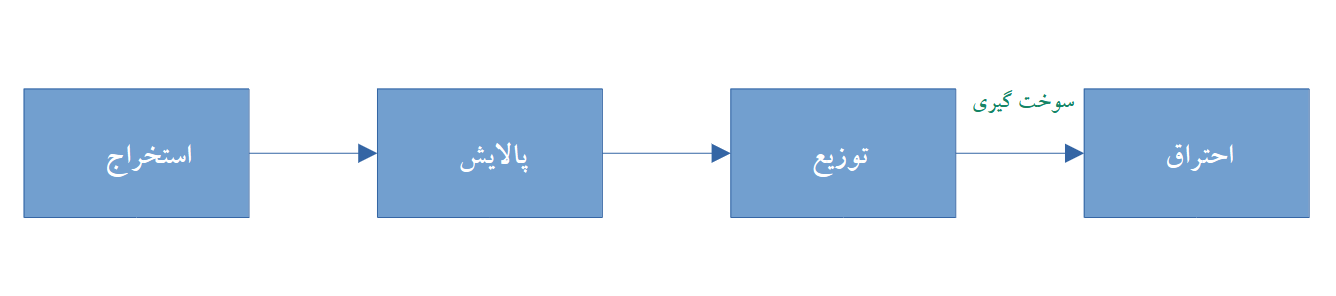
\includegraphics[width=15cm]{Figures/LPG/supply-chain.png}
 	\caption{ زنجیره تأمین سوخت}\label{Suplly-Chain}
 \end{figure}
 
\subsection{تجارت جهانی}
 تقاضای جهانی  
 \lr{LPG }
 در
  \cref{future}
 و تجارت دریایی مرتبط با آن در حال افزایش است. در سال 2022،
  تقاضای جهانی
   \lr{LPG}
    با رشد 
    $\%$5.3
    به رکورد 342 میلیون تن رسید. پیش‌بینی‌ها نشان می‌دهد که حجم تجارت دریایی
    \lr{LPG}
     در سال 2023 حدود 6 میلیون تن افزایش یافته و نسبت به 2022 رشد 5$\%$
   
      داشته است. همچنین، برای سال 2024، رشد
      $\%$3.2
        پیش‌بینی شده و انتظار می‌رود حجم تجارت تا سال 2027 به حدود 142 میلیون تن برسد.
 \begin{figure}[!h]
	\centering
	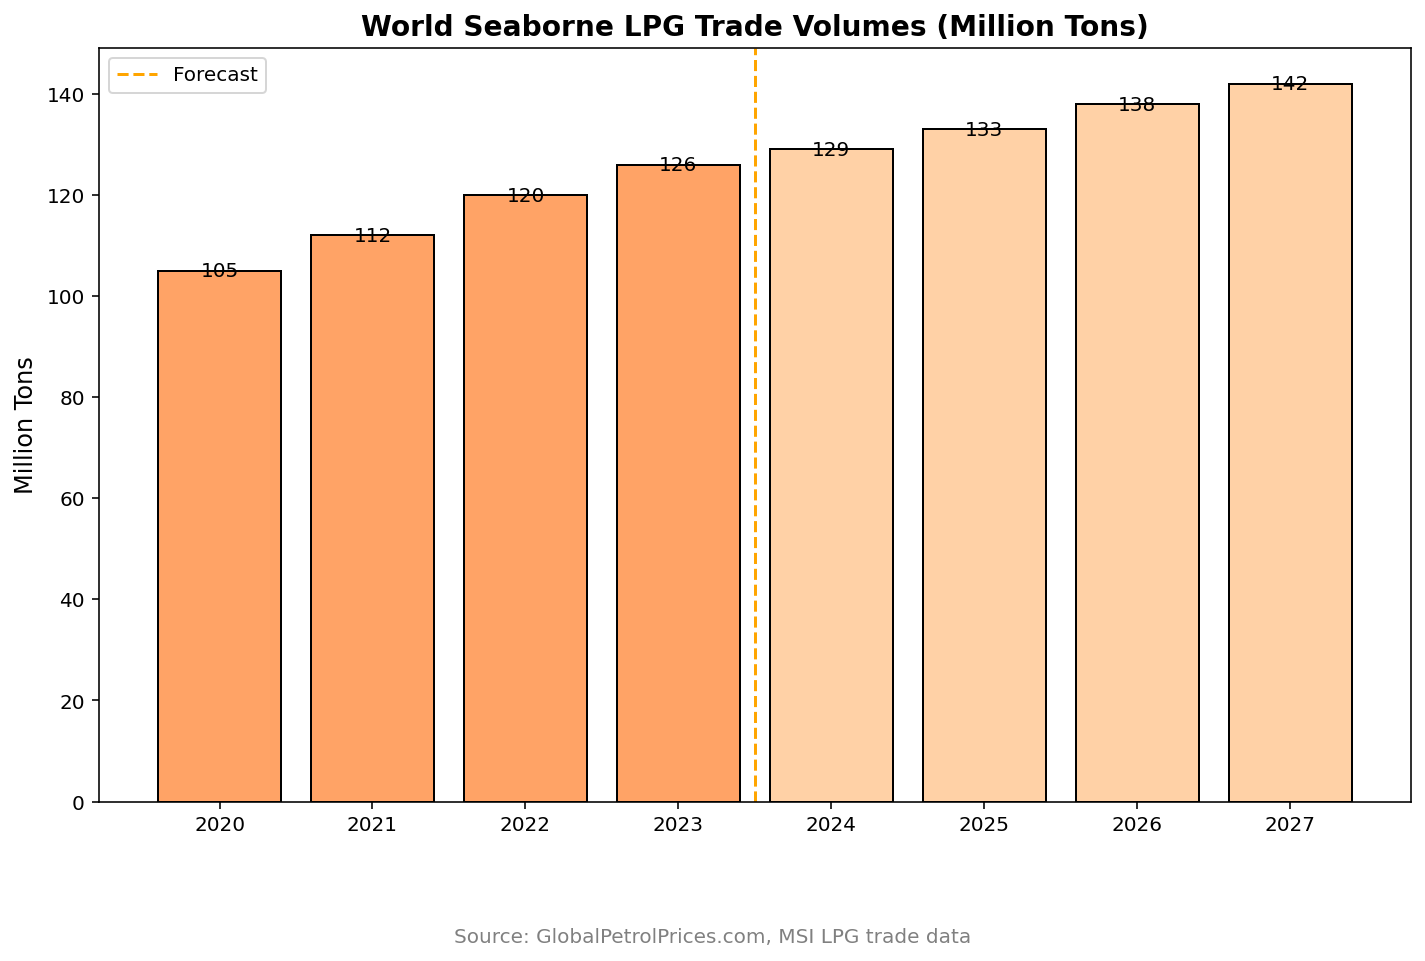
\includegraphics[width=15cm]{Figures/LPG/future.png}
	\caption{ درخواست \lr{LPG}}\label{future}
\end{figure} 
 
\subsection{قیمت سوخت}
استفاده از
 \lr{LPG}
 (گاز مایع) به عنوان سوخت، به‌دلیل قیمت جذاب آن در برخی مناطق مانند ایالات متحده و خلیج فارس، گزینه‌ای اقتصادی برای مالکان و اپراتورها محسوب می‌شود. از نظر هزینه‌های سرمایه‌ای 
 \LTRfootnote{(CAPEX)}،
  \lr{LPG }
 مزایای قابل توجهی نسبت به سایر گزینه‌های سوخت دوگانه 
\LTRfootnote{Dual-Fuel}
  مانند 
  \lr{LNG}
   دارد؛ به‌طوری که ساخت یک کشتی کانتینری ۱۰ هزار 
   \lr{TEU}
   با سوخت 
   \lr{LPG}
    حدود ۱۰۰ میلیون دلار هزینه دارد، یعنی ۲۰$\%$ ارزان‌تر از کشتی مشابه با سوخت 
    \lr{LNG }
    که حدود ۱۲۵ میلیون دلار هزینه می‌برد. همچنین، هزینه تبدیل موتورهای دیزلی به موتورهای دوگانه 
    \lr{LPG }
    (بین ۹.۵ تا ۲۷ میلیون دلار) در مقایسه با تبدیل به
     \lr{LNG}
     (بین ۱۲ تا ۳۳ میلیون دلار) مقرون‌به‌صرفه‌تر است. این عوامل باعث می‌شود.
      \lr{LPG }
      به‌عنوان گزینه‌ای جذاب برای صنعت کشتیرانی مطرح شود.
(\cref{price})
\begin{figure}[!h]
   	\centering
   		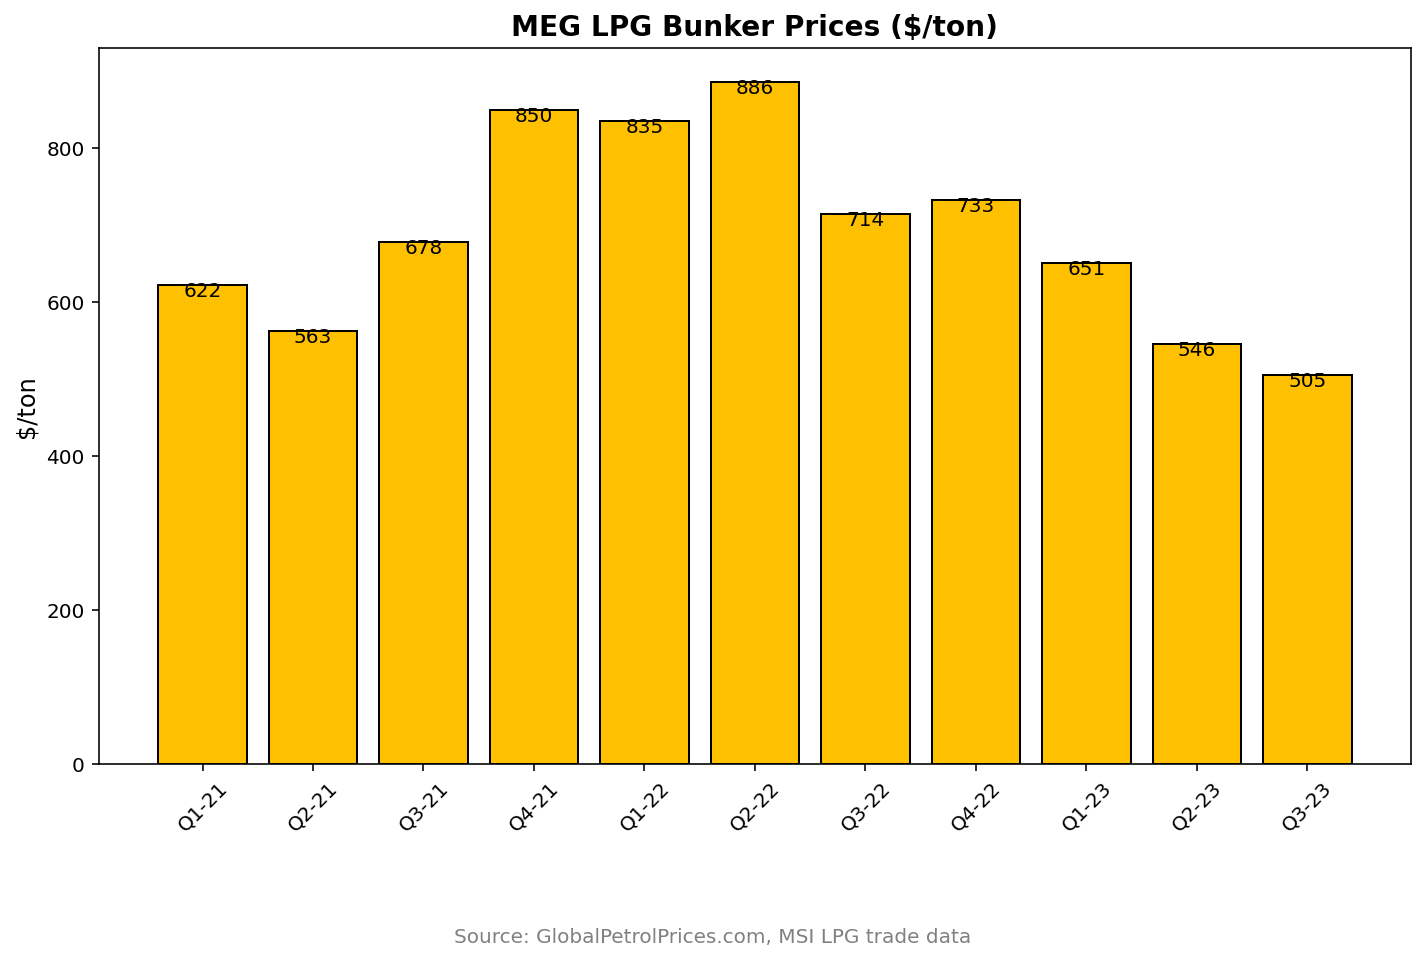
\includegraphics[width=15cm]{Figures/LPG/price.png}
   	\caption{ قیمت سوخت در خلیج فارس}\label{price}
\end{figure}
\\
\\
\subsection{تأمین و نگهداری}
\section{نتیجه‌گیری}
\begin{itemize}
	\item \textbf{مزایای زیست‌محیطی \lr{LPG}:}
	\begin{itemize}
		\item LPG به‌عنوان یک سوخت فسیلی مزیت‌های قابل توجهی در کاهش \textbf{آلودگی هوا} نسبت به سوخت‌های نفتی سنتی (مانند مازوت) دارد.
		\item استفاده از LPG موجب \textbf{کاهش انتشار گازهای گلخانه‌ای} می‌شود، به‌ویژه اگر با فناوری‌های مکملی مانند \textbf{کربن‌گیری در کشتی} همراه شود.
		\item این سوخت می‌تواند با \textbf{مقررات سازمان بین‌المللی دریانوردی (IMO)} درباره کاهش اکسیدهای گوگرد مطابقت داشته باشد و همچنین در بلندمدت با اهداف کربن‌زدایی این سازمان همخوانی داشته باشد.
	\end{itemize}
	
	\item \textbf{پتانسیل LPG برای آینده:}
	\begin{itemize}
		\item استفاده از LPG در بلندمدت به تولید سوخت‌های تجدیدپذیر وابسته است، که انتظار می‌رود با سرعت بالایی افزایش یابد.
		\item با رشد تجارت دریایی و افزایش تقاضا برای LPG، ناوگان جهانی کشتی‌های حمل LPG رشد خواهد کرد و این فرصت برای استفاده از LPG به‌عنوان سوخت افزایش می‌یابد.
		\item زیرساخت‌های حمل‌ونقل، ذخیره‌سازی و استفاده از LPG طی چند دهه به‌خوبی توسعه یافته است.
	\end{itemize}
	
	\item \textbf{چالش‌های موجود:}
	\begin{itemize}
		\item تکنولوژی‌های موتوری برای LPG محدود است. به‌عنوان مثال، هنوز موتور دریایی چهارزمانه‌ای که بتواند از LPG استفاده کند، وجود ندارد، بنابراین موتورهای کمکی کشتی‌ها نیاز به سوخت‌های دیگری برای کربن‌زدایی دارند.
		\item قوانین و چارچوب‌های مقرراتی برای استفاده از LPG به‌عنوان سوخت، خصوصاً در حوزه \textbf{سوخت‌رسانی (bunkering)}، هنوز کامل نیست و فقط راهنماهای اولیه در سطح IMO تدوین شده است.
	\end{itemize}

	\item \textbf{عامل تعیین‌کننده:}
	\begin{itemize}
		\item آینده LPG به‌عنوان یک سوخت مهم در صنعت دریانوردی به سرعت \textbf{کربن‌زدایی تولید LPG} و پیشرفت فناوری‌های مرتبط مانند \textbf{کربن‌گیری} وابسته است.
		\item همچنین LPG ممکن است به‌عنوان یک سوخت \textbf{انتقالی} تا زمان توسعه کامل سوخت‌های بدون کربن یا نزدیک به صفر کربن عمل کند.
	\end{itemize}
\end{itemize}


~
را در فایل 
\verb~AUTthesis.tex~،
غیرفعال%
\RTLfootnote{
برای غیرفعال کردن یک دستور، کافی است پشت آن، یک علامت
\%
 بگذارید.
}
 کنید. زیرا در غیر این صورت، ابتدا مطالب فصل ۱ و ۲ پردازش شده (که به درد ما نمی‌خورد؛ چون ما می‌خواهیم خروجی فصل ۳ را ببینیم) و سپس مطالب فصل ۳ پردازش می‌شود و این کار باعث طولانی شدن زمان اجرا می‌شود. زیرا هر چقدر حجم فایل اجرا شده، بیشتر باشد، زمان بیشتری هم برای اجرای آن، صرف می‌شود.

\subsection{مراجع}
برای وارد کردن مراجع به فصل 2
مراجعه کنید.
\subsection{واژه‌نامه فارسی به انگلیسی و برعکس}
برای وارد کردن واژه‌نامه فارسی به انگلیسی و برعکس، بهتر است مانند روش بکار رفته در فایل‌های 
\verb;dicfa2en;
و
\verb;dicen2fa;
عمل کنید.

\section{اگر سوالی داشتم، از کی بپرسم؟}
برای پرسیدن سوال‌های خود در مورد حروف‌چینی با زی‌پرشین،  می‌توانید به
 \href{http://forum.parsilatex.com}{تالار گفتگوی پارسی‌لاتک}%
\LTRfootnote{\url{http://www.forum.parsilatex.com}}
مراجعه کنید. شما هم می‌توانید روزی به سوال‌های دیگران در این تالار، جواب بدهید.
~
و
\verb~\chapter{سوخت \lr{LPG}}
\section{کلیات}
تا دسامبر ۲۰۲۳، تعداد ۱۶۴۴ کشتی حامل
 \lr{LPG}
 وجود داشت که از میان آن‌ها، ۲۰۴ کشتی بر اساس مدل موتور اصلی نصب‌شده، قابلیت تبدیل به سوخت 
 \lr{LPG }
 را داشتند. این تغییر امکان بهره‌برداری از محموله کشتی‌ها و زیرساخت‌های موجود را فراهم کرده و هزینه‌های عملیاتی آن‌ها را به حداقل می‌رساند. 
به عنوان یک سوخت 
\lr{LPG} 
منحصر به فرد هست،‌ زمانی که از کربن‌‌زدایی در کشتی صحبت می‌کنیم نقش مهم و در حال رشدی 
\lr{LPG}
بازی می‌کند.
\lr{LPG} 
عمدتاً از پروپان و بوتان تشکیل شده که تفاوت‌های جزئی شیمیایی آن‌ها باعث کاربردهای خاص می‌شود.
\lr{LPG}
می‌تواند تحت فشار متوسط در دمای معمول مایع شود، که حمل‌ونقل و ذخیره‌سازی آن را آسان‌تر از سایر سوخت‌های گازی می‌کند.
سوخت 
\lr{LPG} 
به صورت مایع حمل و نگهداری می‌شود، اما به صورت گاز مصرف می‌شود، در حالیکه می‌تواند حمل و نقل دریایی تمیزتر به نسبت  بسیاری از جایگزین‌های موجود در حال حاضر ارائه دهد.

سفارشات کشتی‌های با سوخت 
\lr{LPG}
 رکورد شکن شده است، به طور مثال کشتی‌های
\lr{117 VLGC}
  سفارش داده شده یا در حال ساخت با
\lr{LPG}
   حرکت می‌کنند. و پیش‌بینی می‌شود که 86 درصد از این نوع کشتی‌های  
     جدیدی که در سال‌های آینده وارد بازار می‌شوند، قابلیت کار با 
\lr{LPG}
    را داشته باشند. اگرچه 
 \lr{LPG} 
    در حال حاضر یک سوخت محبوب برای حامل های گاز بزرگ است، این بخش تنها 8 درصد از آلاینده های حمل و نقل را به خود اختصاص می‌دهد و 92 درصد آلاینده‌ها را بقیه کشتی‌ها به جا می‌گذارند. تبدیل این کشتی ها یک فرصت عالی برای کاهش انتشار گازهای گلخانه‌ای جهانی است.
جهان ما به طور فزاینده‌ای به سمت کربن کم‌تر حرکت می‌کند و همه بخش‌های اقتصاد باید به مسئله انتشار گازهای گلخانه‌ای بپردازند.
\newpage

در بخش کشتیرانی،
دلایل استفاده از این سوخت به شرح زیر هست:
\begin{enumerate}
	\item 
	توسعه 
	\lr{LPG}
	 به عنوان سوخت دریایی به گسترش فناوری‌های کاهش کربن وابسته است و پیش‌بینی می‌شود،
	  \lr{rLPG }
	  \LTRfootnote{Refrigerated Liquefied Petroleum Gas}
	  تا سال 2050 تا 50 درصد تقاضای جهانی را پوشش دهد.
	\item 
	\lr{LPG}	
	 با استانداردهای زیست‌محیطی فعلی از جمله 
	 \textbf{محدودیت گوگرد} سازمان بین‌المللی دریانوردی 
	 \lr{IMO}
	  مطابقت دارد.
	\item 
	\lr{LPG} 
	دارای شبکه حمل‌ونقل گسترده‌ای است که شامل بیش از 1600 کشتی حامل 
	\lr{LPG}
	 و بیش از 1000 تأسیسات ذخیره‌سازی است.
	\item  
	می‌تواند عملکرد زیست‌محیطی بخش کشتیرانی را به سرعت بهبود بخشد.
	\item 
	انتشار گازهای مضر آن کم و هزینه آن، مقرون‌به‌صرفه است که به بهبود محیط‌زیست کمک می‌کند.
	\item 
	\lr{LPG}
	 انعطاف‌پذیر است و زنجیره‌های تأمین آن در سراسر جهان موجود است، که باعث می‌شود زیرساخت‌های سوخت‌رسانی راحت‌تر از بسیاری از سوخت‌های جایگزین دیگر پیاده‌سازی شود.
	 \item 
	 برای سیستم‌های پیشران مبتنی بر
	  \lr{LPG}
هیچ محدودیت یا مانع فناورانه‌ای وجود ندارد.
	 \item	
	  \lr{LPG}
	  به فناوری جدید یا پیشرفته نیاز ندارد و آماده بهره‌برداری است.
	 \item 
	 چه برای بزرگ‌ترین کشتی‌های جهان و چه برای کوچک‌ترین موتورهای قایق،
	  \lr{LPG} 
	  امروز یک سوخت کم‌کربن و کم‌انتشار ارائه می‌دهد، و با معرفی 
	  \lr{LPG} 
	  تجدیدپذیر، کربن‌زدایی کم‌هزینه در آینده امکان‌پذیر می‌شود.
\end{enumerate}
	 
\newpage

\begin{table}[h!]
	\centering
	\caption{مشخصات سوخت \lr{LPG}}
	\label{dsd}
	\begin{tabular}{|m{2cm}|m{12cm}|}
		\hline
		\textbf{مشخصه} & \textbf{توضیحات} \\
		\hline
		دمای جوش   & $-42$ درجه (پروپان خالص) و $-0.5$ درجه (بوتان خالص) \\
		فشار بخار & $1.8$ بار (بوتان خالص) تا $7.3$ بار (پروپان خالص) در دمای 15 درجه\\
		 چگالی & $1.89$ کیلوگرم بر متر مکعب (پروپان خالص) تا $2.54$ کیلوگرم بر متر مکعب (بوتان خالص) در دمای $15$ ‌درجه \\
		حداقل انرژی احتراق & $ 0.25 mj$\\
		چگالی انرژی حجمی &  $  26.5MJ/L $   \\
		نسبت اندازه مخزن & $1.5$  \\
		\hline
	\end{tabular}
\end{table}

\section{اثرات زیست محیطی}
	\subsection{مزایا}
	گاز مایع \lr{(LPG)} یکی از پاک‌ترین سوخت‌های فسیلی موجود است که مزایای زیست‌محیطی و سلامتی بسیاری دارد. در این متن به بررسی برخی از این مزایا می‌پردازیم.
	\cite{Newes2023}
	\begin{itemize}
		\item \lr{LPG} یک سوخت غیرسمی است و تأثیر منفی روی خاک، آب و سفره‌های آب زیرزمینی ندارد.
		\item این سوخت به بهبود کیفیت هوای داخل و خارج از ساختمان کمک می‌کند، زیرا ذرات معلق و اکسیدهای نیتروژن \lr{(NOX)} کمتری نسبت به سوخت‌هایی مانند دیزل، نفت، چوب یا زغال‌سنگ تولید می‌کند.
		\item \lr{LPG} نقش مهمی در کاهش انتشار دی‌اکسید کربن و سایر گازهای گلخانه‌ای دارد.
		\item ردپای کربنی \lr{LPG} بیش از ۲۰ $\%$ کمتر از بنزین و بیش از ۱۰$\%$ کمتر از دیزل است.
		\item \lr{LPG} به کاهش انتشار کربن سیاه کمک می‌کند. کربن سیاه دومین عامل بزرگ گرمایش جهانی است و می‌تواند مشکلات جدی برای سلامت انسان ایجاد کند.
		\item \lr{LPG} در زمینه‌های مختلفی مانند حمل‌ونقل، پخت‌وپز، گرمایش، فرآیندهای صنعتی و تولید برق محلی کاربرد دارد.
		\item به‌عنوان یک سوخت کم‌کربن، جایگزین مناسبی برای سوخت‌های سنتی در مقیاس‌های کوچک و متوسط است.
	\end{itemize}
	\subsection{معایب}
	به طور کلی، اگرچه 
	\lr{LPG} 
	از نظر تولید آلاینده‌های کلاسیک مانند ذرات معلق مزایایی دارد، اما چالش‌های زیست‌محیطی مربوط به ذخیره‌سازی و نشت آن، نیازمند مدیریت دقیق و نظارت مستمر هستند.
	\begin{itemize}
		\item 
	نیاز به مخازن ذخیره‌سازی مقاوم و ایمن برای
	 \lr{LPG}
	 تأثیرات زیست‌محیطی قابل توجهی دارد، زیرا تولید و نگهداری این مخازن مستلزم مصرف بالای مواد اولیه مانند فولادهای آلیاژی و استفاده از فرآیندهای صنعتی پرانرژی مانند جوشکاری و شکل‌دهی است که منجر به افزایش انتشار گازهای گلخانه‌ای
\lr{(CO2)}
	   و آلاینده‌های صنعتی می‌شود. علاوه بر این، خطر نشت و تشکیل ابرهای گازی ناشی از 
\lr{LPG}
	   می‌تواند باعث کاهش کیفیت هوا شده و در صورت ترکیب با سایر آلاینده‌ها، به تشکیل مه‌دود فتوشیمیایی کمک کند، که این امر سلامت اکوسیستم‌های ساحلی و دریایی را تهدید می‌کند.
		\item 
اثر زیست‌محیطی نشت 
\lr{LPG}
 و تشکیل ابرهای گازی در صورتی که
  \lr{LPG}
  نشت کند، این گاز به دلیل چگالی بالاتر از هوا، در سطح زمین یا آب‌های سطحی پخش می‌شود. این امر می‌تواند موجب کاهش کیفیت هوا و افزایش خطر آتش‌سوزی شود. 
\lr{LPG}
  به طور مستقیم اثر گلخانه‌ای قابل توجهی ندارد، اما در ترکیب با آلاینده‌های دیگر می‌تواند به تشکیل مه‌دود فتوشیمیایی کمک کند که کیفیت هوا را کاهش داده و سلامت اکوسیستم‌های ساحلی و دریایی را تهدید می‌کند. همچنین، در صورت نشت در آب، ممکن است اثرات نامطلوبی بر حیات آبزیان داشته باشد.
  \cite{osmthome}
	\end{itemize}

\section{تکنولوژی‌های مرتبط با \lr{LPG}}
\subsection{تکنولوژی تولید}
\subsection{تکنولوژی استفاده در کشتی}
\subsection{ایمنی و الزامات فنی }
ذخیره‌سازی، استفاده و حمل‌ونقل
 \lr{LPG}
 خطرات بالقوه‌ای را به همراه دارد که باید در تمامی سناریوهای صنعتی کاهش یابد. در زمینه سوخت دریایی، برای مقابله با این خطرات، اجرای تدابیری در طراحی و ساخت کشتی، تنظیمات ماشین‌آلات و فناوری‌ها، فناوری‌های سوخت‌رسانی، رویه‌های داخلی کشتی و آموزش خدمه ضروری است.
\subsubsection{سنگینی نسبت به هوا}
\lr{LPG}
به صورت گازی تقریباً دو برابر سنگین‌تر از هوا است. این ویژگی باعث می‌شود که در سطوح پایین‌تر جمع شود و خطراتی را در مکان‌های بسته یا گودال‌ها ایجاد کند.تهویه مناسب در سطوح پایین و فضاهای بسته الزامی است.
همچنین استفاده از آشکارسازهای گاز در نزدیکی زمین برای شناسایی نشت گاز الزامی هست.
\subsubsection{مخلوط قابل اشتعال  با هوا}
\lr{LPG}
در غلظت 2 تا 10 درصد با هوا مخلوط قابل اشتعالی تشکیل می‌دهد. در صورت ذخیره یا استفاده نادرست، خطر آتش‌سوزی و انفجار وجود دارد.دوری از منابع گرما، جرقه و شعله باز.
استفاده از تجهیزات ضد انفجار در محل ذخیره یا استفاده.
\subsubsection{تأثیرات استنشاق در غلظت‌های بالا}
در غلظت‌های بسیار بالا، 
\lr{LPG}
 می‌تواند اثرات بی‌هوشی و خفگی داشته باشد زیرا اکسیژن موجود در هوا را رقیق می‌کند.اطمینان از وجود تهویه کافی در فضاهای بسته.
 استفاده از ماسک‌های تنفسی مناسب در شرایط اضطراری.
\subsubsection{سوختگی‌های ناشی از مایع}
 مایع به دلیل تبخیر سریع باعث سوختگی شدید سرد می‌شود. همچنین، تبخیر می‌تواند تجهیزات را به حدی سرد کند که خطر سوختگی را افزایش دهد.
 استفاده از دستکش و لباس‌های محافظ در هنگام کار با 
 \lr{LPG}
  مایع.
 عایق‌کاری مناسب تجهیزات برای جلوگیری از تماس مستقیم.
\subsubsection{احتراق مخلوط بخار/هوا در اثر نشت}
مخلوط بخار 
\lr{LPG}
و هوا می‌تواند در فاصله‌ای دورتر از نقطه نشت آتش بگیرد و شعله به منبع نشت بازگردد.بررسی منظم و رفع نشتی تجهیزات ذخیره و انتقال \lr{LPG}.
نصب شیرهای خودکار قطع گاز برای جلوگیری از گسترش شعله.
\subsubsection{خطرات مخازن خالی}
مخزن خالی
 \lr{LPG}
  ممکن است همچنان حاوی بخار
\lr{\textbf{LPG}}
تخلیه و تهویه کامل مخازن قبل از انجام هرگونه تعمیرات.
برچسب‌گذاری مخازن برای هشدار به افراد از خطرات احتمالی.
\subsection{سیستم‌های ذخیره‌سازی و مدیریت 
	\lr{LPG} 
	در کشتی‌ها}
سوخت‌رسانی
 \lr{LPG}
  به کشتی‌ها به‌عنوان یک سوخت دریایی مزایا و خطراتی دارد. 
   \lr{LPG}
   در حالت مایع خود قابل اشتعال یا انفجار نیست، نشت آن می‌تواند باعث ایجاد بخارهایی شود که به راحتی با باد پراکنده و در صورت برخورد با منبع حرارتی ممکن است آتش بگیرند. همچنین، نشت
    \lr{LPG}
    روی آب می‌تواند منجر به استخر آتش\LTRfootnote{\lr{pool fire}}
     شود که بسیار داغ‌تر و سریع‌تر از آتش‌های ناشی از نفت یا بنزین می‌سوزد و قابل خاموش شدن نیست. در عملیات سوخت‌رسانی، نشت 
    \lr{LPG}
    می‌تواند خطرات زیادی از جمله آتش‌سوزی یا انفجار در مناطق بندری ایجاد کند. به همین دلیل، تدابیر ایمنی ویژه‌ای مانند استفاده از لوله‌های دو جداره و آشکارسازهای هیدروکربنی برای جلوگیری از نشت و آسیب به کشتی‌ها ضروری است. با این حال، سوخت‌رسانی
     \lr{LPG}
     هنوز چارچوب نظارتی رسمی و دستورالعمل‌های مشخصی ندارد و توسعه این دستورالعمل‌ها می‌تواند به بهبود ایمنی، کارایی و آگاهی محیط‌زیستی کمک کند، مشابه آنچه برای دیگر سوخت‌ها مانند 
     \lr{LNG }
     انجام شده است.
\subsection{ایمنی و الزامات فنی مرتبط با حمل }
برای بهبود ایمنی و کارایی در سوخت‌گیری \lr{LPG}، لازم است استانداردها و مشخصات فنی تجهیزات مانند شیلنگ‌ها، نازل‌ها و شیرآلات تدوین شود و معیارهای عملکرد و الزامات ایمنی آن‌ها تعریف گردد. روال‌هایی برای تست و صدور گواهی تجهیزات سوخت‌گیری ایجاد شده و همراه با مستندات و مواد آموزشی جامع، در اختیار ذینفعان از جمله اپراتورها و خدمه قرار گیرد. پروژه‌های آزمایشی و نمایش‌های عملی به منظور اعتبارسنجی چارچوب‌ها و شناسایی شکاف‌ها یا مشکلات احتمالی اجرا شده و از نتایج آن برای اصلاح رویه‌ها و ارتقای ایمنی استفاده شود.

این فرآیندها تضمین می‌کند که تمامی تجهیزات و عملیات مرتبط با سوخت‌گیری \lr{LPG} مطابق با استانداردهای بین‌المللی بوده و صدور گواهی‌ها به ایمنی جهانی کمک کند.
\\
فرآیند سوخت‌گیری در سه مرحله انجام می‌شود.
\subsubsection{مرحله قبل از سوخت‌گیری }
مرحله پیش از سوخت‌گیری 
\LTRfootnote{\lr{Before bunkering}}
	 از سفارش سوخت آغاز شده و با شروع فرآیند سوخت‌گیری خاتمه می‌یابد.  
در این مرحله آمادگی، انجام تمام اقدامات لازم برای اطمینان از انتقال ایمن سوخت بسیار مهم است. این اقدامات شامل موارد زیر می‌شوند:

\begin{itemize}
	\item اطمینان از اینکه تمامی یافته‌های ارزیابی ریسک به درستی مورد توجه قرار گرفته‌اند.
	\item ارزیابی سازگاری بین کشتی دریافت‌کننده سوخت و تأسیسات .
	\item تهیه و توافق بر روی برنامه واکنش اضطراری.
	\item ارائه دستورالعمل‌های ایمنی و آموزش کارکنان .
	\item هماهنگی با نهادهای مسئول برای دریافت مجوزهای لازم.
	\item ارزیابی فرآیندهای مرتبط دیگر، مانند عملیات هم‌زمان \LTRfootnote{\lr{SIMOPS}}.
	\item تعیین جزئیات عملیاتی مانند نرخ انتقال، محدودیت‌های بارگیری،  
	خاموشی اضطراری
	\LTRfootnote{\lr{ESD}}
	، سیستم ایمنی اضطراری
	\LTRfootnote{ERS} 
	و غیره.
	\item تکمیل تمامی چک‌لیست‌های مورد نیاز پیش از سوخت‌گیری.
\end{itemize}

\subsection{مرحله سوخت‌گیری}

فرآیند سوخت‌رسانی
\LTRfootnote{During bunkering}
 با اتصال کشتی دریافت‌کننده به تأسیسات سوخت‌رسانی آغاز می‌شود و با انتقال واقعی سوخت ادامه می‌یابد، و با اقدامات لازم برای بستن ایمن شیر از تأسیسات سوخت‌رسانی خاتمه می‌یابد.  
در طول مرحله سوخت‌گیری، بخش‌های حیاتی سیستم باید به طور مداوم کنترل شوند، از جمله:

\begin{itemize}
	\item سطح مخازن؛
	\item فشار مخازن؛
	\item دمای مخازن؛
	\item نرخ انتقال پمپ؛
	\item نرخ جریان پمپ؛
	\item عملیات سیستم‌های \lr{ESD} و \lr{ERS}؛
	\item تنظیم خطوط پهلوگیری و شیلنگ‌ها؛
	\item نظارت و حفظ سایر جنبه‌های ایمنی، مانند مناطق ایمنی.
\end{itemize}

\subsection{پس‌از سوخت‌گیری}
پس از اتمام سوخت‌گیری
\LTRfootnote{After bunkering}
، باید به نکات زیر توجه شود:
\begin{itemize}
	\item انجام موفقیت‌آمیز فرآیندهای سیستمی ، مانند تبخیر خطوط و خنثی‌سازی گازها در خطوط و شیلنگ‌ها، بدون انتشار گاز به جو.
	\item قطع ایمن ارتباط بین کشتی دریافت‌کننده و تأسیسات سوخت‌رسانی.
	\item جداسازی ایمن کشتی دریافت‌کننده یا کشتی سوخت‌رسان از کشتی دریافت‌کننده و اطلاع‌رسانی به مقامات بندری.
\end{itemize}

\section{الزامات قانونی}
برای کاهش ریسک‌های مرتبط با کشتی، خدمه و محیط زیست، کدهای ایمنی بین‌المللی پیش‌نیازهای لازم برای تجهیزات، ماشین‌آلات و سیستم‌های کشتی را تعیین می‌کنند. این الزامات شامل استانداردهای عملکردی، ارزیابی ریسک، مقررات و نیازمندی‌های عملیاتی است که همراه با آموزش مناسب خدمه، ایمنی عملیات کشتی را تضمین می‌کنند.
\subsection{کد \lr{IGC}}
این کد مرتبط با ساخت و تجهیز کشتی‌هایی که گاز مایع شده را به صورت فله حمل می‌کنند و استفاده از این گازها به‌عنوان سوخت هست.
\subsection{کد \lr{IGF}}
این کد مخصوص کشتی‌های غیرحامل گاز که از گاز یا سوخت‌های با نقطه اشتعال پایین، مانند
\lr{LPG}،
به‌عنوان سوخت استفاده می‌کنند.	

\subsection{استاندارد \lr{MSC.1/Circ.1666}}
استاندارد ایمنی برای کشتی‌هایی که از ال پی جی به‌عنوان سوخت استفاده می‌کنند.
...
\subsection{استاندارد \lr{MSC.1/Circ.1679}}
...راهنمایی‌های موقت برای استفاده از محموله ال پی جی به‌عنوان سوخت.


\section{اقتصاد و بازار \lr{LPG}}
\subsection{چرخه عمر}
دستورالعمل‌های چرخه عمر گازهای گلخانه‌ای 
\LTRfootnote{\lr{LCA}}
 سازمان بین‌المللی دریانوردی  برای سوخت‌های دریایی، شامل 
 \lr{LPG}
 ، ابتدا در نشست 
 \lr{MEPC 80 (MEPC.376(80))}
 تصویب شدند و تمامی مراحل زنجیره تأمین این سوخت را پوشش می‌دهند. در نشست
  \lr{MEPC 81}،
   نسخه
    \lr{2024}
    این دستورالعمل‌ها 
  \lr{  (MEPC.391(81)) }
    با اصلاح عوامل توزیع پیش‌فرض، به‌روزرسانی الگوی عوامل توزیع از چاه به مخزن
    \LTRfootnote{Well-to-Tank}
    \cref{Suplly-Chain}
     و اضافه‌شدن الگوی جدید برای عوامل توزیع از مخزن به مصرف 
\LTRfootnote{Tank-to-Wake}
      بازنگری شد.
 \cite{Comparative-Life-Cycle}
 \begin{figure}[!h]
 	\centering
 	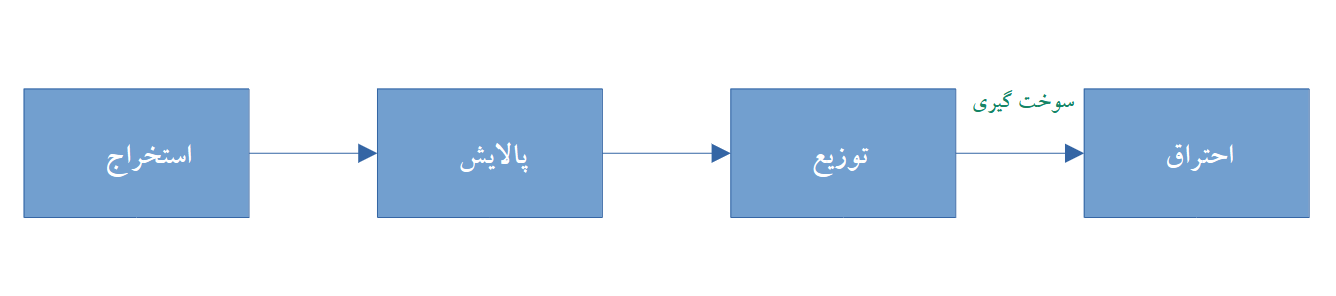
\includegraphics[width=15cm]{Figures/LPG/supply-chain.png}
 	\caption{ زنجیره تأمین سوخت}\label{Suplly-Chain}
 \end{figure}
 
\subsection{تجارت جهانی}
 تقاضای جهانی  
 \lr{LPG }
 در
  \cref{future}
 و تجارت دریایی مرتبط با آن در حال افزایش است. در سال 2022،
  تقاضای جهانی
   \lr{LPG}
    با رشد 
    $\%$5.3
    به رکورد 342 میلیون تن رسید. پیش‌بینی‌ها نشان می‌دهد که حجم تجارت دریایی
    \lr{LPG}
     در سال 2023 حدود 6 میلیون تن افزایش یافته و نسبت به 2022 رشد 5$\%$
   
      داشته است. همچنین، برای سال 2024، رشد
      $\%$3.2
        پیش‌بینی شده و انتظار می‌رود حجم تجارت تا سال 2027 به حدود 142 میلیون تن برسد.
 \begin{figure}[!h]
	\centering
	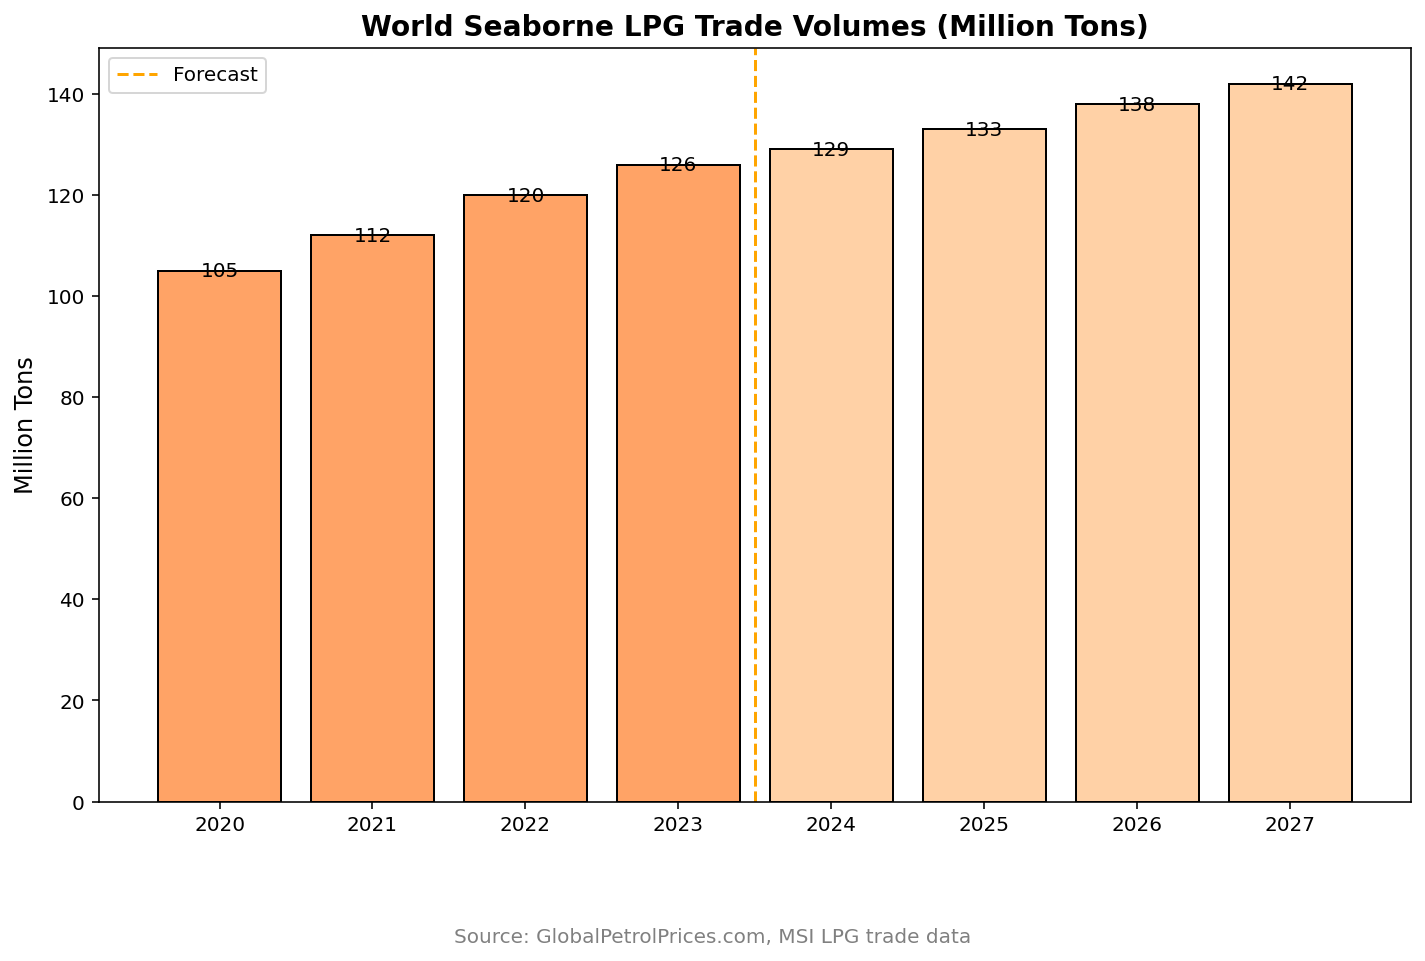
\includegraphics[width=15cm]{Figures/LPG/future.png}
	\caption{ درخواست \lr{LPG}}\label{future}
\end{figure} 
 
\subsection{قیمت سوخت}
استفاده از
 \lr{LPG}
 (گاز مایع) به عنوان سوخت، به‌دلیل قیمت جذاب آن در برخی مناطق مانند ایالات متحده و خلیج فارس، گزینه‌ای اقتصادی برای مالکان و اپراتورها محسوب می‌شود. از نظر هزینه‌های سرمایه‌ای 
 \LTRfootnote{(CAPEX)}،
  \lr{LPG }
 مزایای قابل توجهی نسبت به سایر گزینه‌های سوخت دوگانه 
\LTRfootnote{Dual-Fuel}
  مانند 
  \lr{LNG}
   دارد؛ به‌طوری که ساخت یک کشتی کانتینری ۱۰ هزار 
   \lr{TEU}
   با سوخت 
   \lr{LPG}
    حدود ۱۰۰ میلیون دلار هزینه دارد، یعنی ۲۰$\%$ ارزان‌تر از کشتی مشابه با سوخت 
    \lr{LNG }
    که حدود ۱۲۵ میلیون دلار هزینه می‌برد. همچنین، هزینه تبدیل موتورهای دیزلی به موتورهای دوگانه 
    \lr{LPG }
    (بین ۹.۵ تا ۲۷ میلیون دلار) در مقایسه با تبدیل به
     \lr{LNG}
     (بین ۱۲ تا ۳۳ میلیون دلار) مقرون‌به‌صرفه‌تر است. این عوامل باعث می‌شود.
      \lr{LPG }
      به‌عنوان گزینه‌ای جذاب برای صنعت کشتیرانی مطرح شود.
(\cref{price})
\begin{figure}[!h]
   	\centering
   		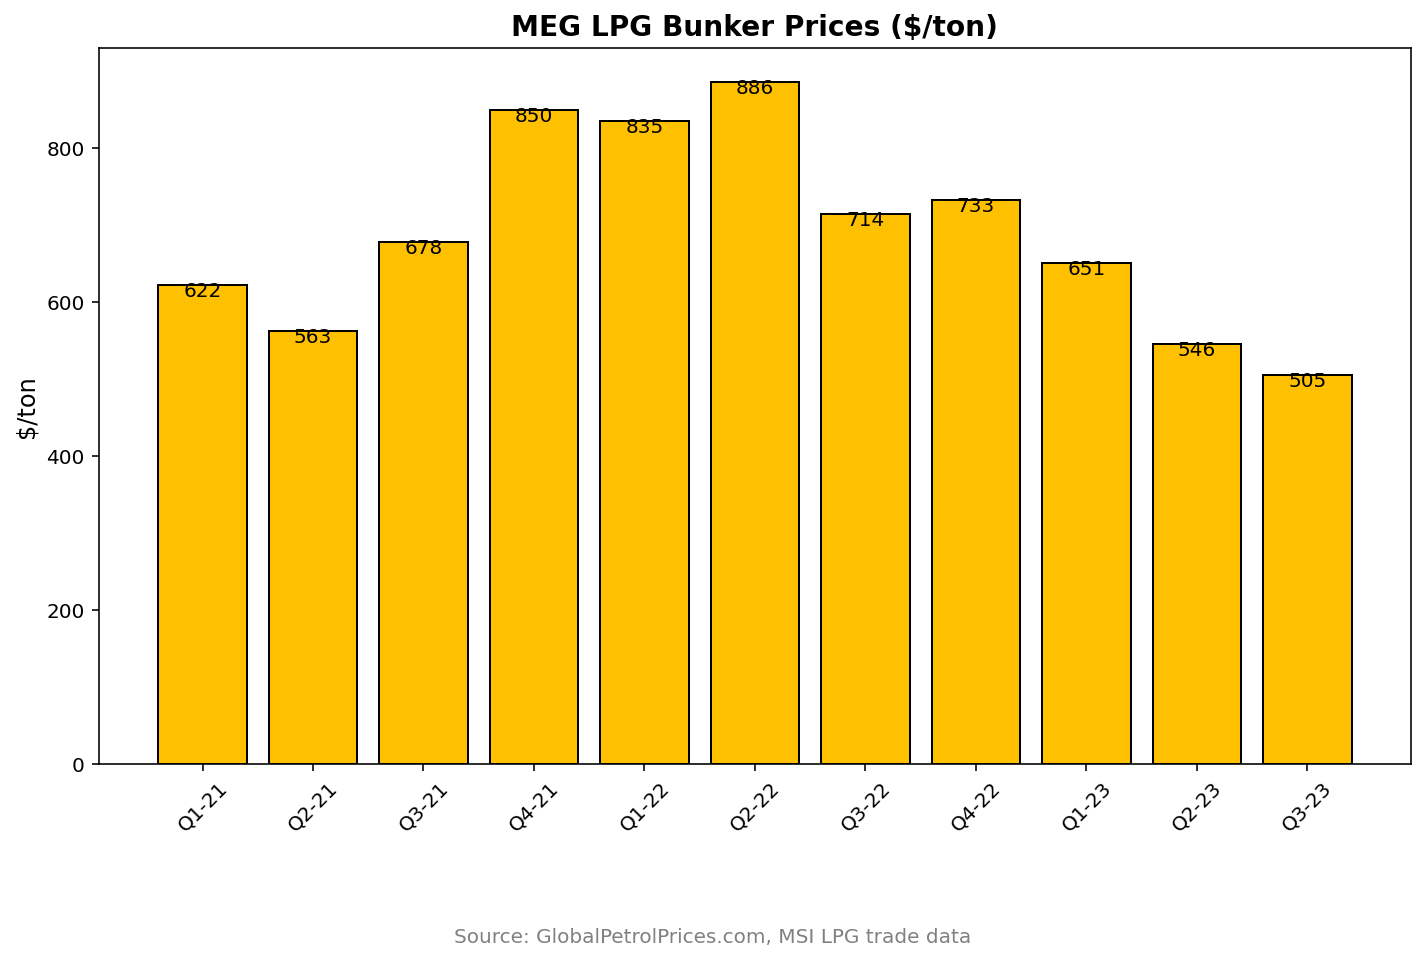
\includegraphics[width=15cm]{Figures/LPG/price.png}
   	\caption{ قیمت سوخت در خلیج فارس}\label{price}
\end{figure}
\\
\\
\subsection{تأمین و نگهداری}
\section{نتیجه‌گیری}
\begin{itemize}
	\item \textbf{مزایای زیست‌محیطی \lr{LPG}:}
	\begin{itemize}
		\item LPG به‌عنوان یک سوخت فسیلی مزیت‌های قابل توجهی در کاهش \textbf{آلودگی هوا} نسبت به سوخت‌های نفتی سنتی (مانند مازوت) دارد.
		\item استفاده از LPG موجب \textbf{کاهش انتشار گازهای گلخانه‌ای} می‌شود، به‌ویژه اگر با فناوری‌های مکملی مانند \textbf{کربن‌گیری در کشتی} همراه شود.
		\item این سوخت می‌تواند با \textbf{مقررات سازمان بین‌المللی دریانوردی (IMO)} درباره کاهش اکسیدهای گوگرد مطابقت داشته باشد و همچنین در بلندمدت با اهداف کربن‌زدایی این سازمان همخوانی داشته باشد.
	\end{itemize}
	
	\item \textbf{پتانسیل LPG برای آینده:}
	\begin{itemize}
		\item استفاده از LPG در بلندمدت به تولید سوخت‌های تجدیدپذیر وابسته است، که انتظار می‌رود با سرعت بالایی افزایش یابد.
		\item با رشد تجارت دریایی و افزایش تقاضا برای LPG، ناوگان جهانی کشتی‌های حمل LPG رشد خواهد کرد و این فرصت برای استفاده از LPG به‌عنوان سوخت افزایش می‌یابد.
		\item زیرساخت‌های حمل‌ونقل، ذخیره‌سازی و استفاده از LPG طی چند دهه به‌خوبی توسعه یافته است.
	\end{itemize}
	
	\item \textbf{چالش‌های موجود:}
	\begin{itemize}
		\item تکنولوژی‌های موتوری برای LPG محدود است. به‌عنوان مثال، هنوز موتور دریایی چهارزمانه‌ای که بتواند از LPG استفاده کند، وجود ندارد، بنابراین موتورهای کمکی کشتی‌ها نیاز به سوخت‌های دیگری برای کربن‌زدایی دارند.
		\item قوانین و چارچوب‌های مقرراتی برای استفاده از LPG به‌عنوان سوخت، خصوصاً در حوزه \textbf{سوخت‌رسانی (bunkering)}، هنوز کامل نیست و فقط راهنماهای اولیه در سطح IMO تدوین شده است.
	\end{itemize}

	\item \textbf{عامل تعیین‌کننده:}
	\begin{itemize}
		\item آینده LPG به‌عنوان یک سوخت مهم در صنعت دریانوردی به سرعت \textbf{کربن‌زدایی تولید LPG} و پیشرفت فناوری‌های مرتبط مانند \textbf{کربن‌گیری} وابسته است.
		\item همچنین LPG ممکن است به‌عنوان یک سوخت \textbf{انتقالی} تا زمان توسعه کامل سوخت‌های بدون کربن یا نزدیک به صفر کربن عمل کند.
	\end{itemize}
\end{itemize}


~
را در فایل 
\verb~AUTthesis.tex~،
غیرفعال%
\RTLfootnote{
برای غیرفعال کردن یک دستور، کافی است پشت آن، یک علامت
\%
 بگذارید.
}
 کنید. زیرا در غیر این صورت، ابتدا مطالب فصل ۱ و ۲ پردازش شده (که به درد ما نمی‌خورد؛ چون ما می‌خواهیم خروجی فصل ۳ را ببینیم) و سپس مطالب فصل ۳ پردازش می‌شود و این کار باعث طولانی شدن زمان اجرا می‌شود. زیرا هر چقدر حجم فایل اجرا شده، بیشتر باشد، زمان بیشتری هم برای اجرای آن، صرف می‌شود.

\subsection{مراجع}
برای وارد کردن مراجع به فصل 2
مراجعه کنید.
\subsection{واژه‌نامه فارسی به انگلیسی و برعکس}
برای وارد کردن واژه‌نامه فارسی به انگلیسی و برعکس، بهتر است مانند روش بکار رفته در فایل‌های 
\verb;dicfa2en;
و
\verb;dicen2fa;
عمل کنید.

\section{اگر سوالی داشتم، از کی بپرسم؟}
برای پرسیدن سوال‌های خود در مورد حروف‌چینی با زی‌پرشین،  می‌توانید به
 \href{http://forum.parsilatex.com}{تالار گفتگوی پارسی‌لاتک}%
\LTRfootnote{\url{http://www.forum.parsilatex.com}}
مراجعه کنید. شما هم می‌توانید روزی به سوال‌های دیگران در این تالار، جواب بدهید.

\chapter{سوخت \lr{LPG}}
\section{کلیات}
تا دسامبر ۲۰۲۳، تعداد ۱۶۴۴ کشتی حامل
 \lr{LPG}
 وجود داشت که از میان آن‌ها، ۲۰۴ کشتی بر اساس مدل موتور اصلی نصب‌شده، قابلیت تبدیل به سوخت 
 \lr{LPG }
 را داشتند. این تغییر امکان بهره‌برداری از محموله کشتی‌ها و زیرساخت‌های موجود را فراهم کرده و هزینه‌های عملیاتی آن‌ها را به حداقل می‌رساند. 
به عنوان یک سوخت 
\lr{LPG} 
منحصر به فرد هست،‌ زمانی که از کربن‌‌زدایی در کشتی صحبت می‌کنیم نقش مهم و در حال رشدی 
\lr{LPG}
بازی می‌کند.
\lr{LPG} 
عمدتاً از پروپان و بوتان تشکیل شده که تفاوت‌های جزئی شیمیایی آن‌ها باعث کاربردهای خاص می‌شود.
\lr{LPG}
می‌تواند تحت فشار متوسط در دمای معمول مایع شود، که حمل‌ونقل و ذخیره‌سازی آن را آسان‌تر از سایر سوخت‌های گازی می‌کند.
سوخت 
\lr{LPG} 
به صورت مایع حمل و نگهداری می‌شود، اما به صورت گاز مصرف می‌شود، در حالیکه می‌تواند حمل و نقل دریایی تمیزتر به نسبت  بسیاری از جایگزین‌های موجود در حال حاضر ارائه دهد.

سفارشات کشتی‌های با سوخت 
\lr{LPG}
 رکورد شکن شده است، به طور مثال کشتی‌های
\lr{117 VLGC}
  سفارش داده شده یا در حال ساخت با
\lr{LPG}
   حرکت می‌کنند. و پیش‌بینی می‌شود که 86 درصد از این نوع کشتی‌های  
     جدیدی که در سال‌های آینده وارد بازار می‌شوند، قابلیت کار با 
\lr{LPG}
    را داشته باشند. اگرچه 
 \lr{LPG} 
    در حال حاضر یک سوخت محبوب برای حامل های گاز بزرگ است، این بخش تنها 8 درصد از آلاینده های حمل و نقل را به خود اختصاص می‌دهد و 92 درصد آلاینده‌ها را بقیه کشتی‌ها به جا می‌گذارند. تبدیل این کشتی ها یک فرصت عالی برای کاهش انتشار گازهای گلخانه‌ای جهانی است.
جهان ما به طور فزاینده‌ای به سمت کربن کم‌تر حرکت می‌کند و همه بخش‌های اقتصاد باید به مسئله انتشار گازهای گلخانه‌ای بپردازند.
\newpage

در بخش کشتیرانی،
دلایل استفاده از این سوخت به شرح زیر هست:
\begin{enumerate}
	\item 
	توسعه 
	\lr{LPG}
	 به عنوان سوخت دریایی به گسترش فناوری‌های کاهش کربن وابسته است و پیش‌بینی می‌شود،
	  \lr{rLPG }
	  \LTRfootnote{Refrigerated Liquefied Petroleum Gas}
	  تا سال 2050 تا 50 درصد تقاضای جهانی را پوشش دهد.
	\item 
	\lr{LPG}	
	 با استانداردهای زیست‌محیطی فعلی از جمله 
	 \textbf{محدودیت گوگرد} سازمان بین‌المللی دریانوردی 
	 \lr{IMO}
	  مطابقت دارد.
	\item 
	\lr{LPG} 
	دارای شبکه حمل‌ونقل گسترده‌ای است که شامل بیش از 1600 کشتی حامل 
	\lr{LPG}
	 و بیش از 1000 تأسیسات ذخیره‌سازی است.
	\item  
	می‌تواند عملکرد زیست‌محیطی بخش کشتیرانی را به سرعت بهبود بخشد.
	\item 
	انتشار گازهای مضر آن کم و هزینه آن، مقرون‌به‌صرفه است که به بهبود محیط‌زیست کمک می‌کند.
	\item 
	\lr{LPG}
	 انعطاف‌پذیر است و زنجیره‌های تأمین آن در سراسر جهان موجود است، که باعث می‌شود زیرساخت‌های سوخت‌رسانی راحت‌تر از بسیاری از سوخت‌های جایگزین دیگر پیاده‌سازی شود.
	 \item 
	 برای سیستم‌های پیشران مبتنی بر
	  \lr{LPG}
هیچ محدودیت یا مانع فناورانه‌ای وجود ندارد.
	 \item	
	  \lr{LPG}
	  به فناوری جدید یا پیشرفته نیاز ندارد و آماده بهره‌برداری است.
	 \item 
	 چه برای بزرگ‌ترین کشتی‌های جهان و چه برای کوچک‌ترین موتورهای قایق،
	  \lr{LPG} 
	  امروز یک سوخت کم‌کربن و کم‌انتشار ارائه می‌دهد، و با معرفی 
	  \lr{LPG} 
	  تجدیدپذیر، کربن‌زدایی کم‌هزینه در آینده امکان‌پذیر می‌شود.
\end{enumerate}
	 
\newpage

\begin{table}[h!]
	\centering
	\caption{مشخصات سوخت \lr{LPG}}
	\label{dsd}
	\begin{tabular}{|m{2cm}|m{12cm}|}
		\hline
		\textbf{مشخصه} & \textbf{توضیحات} \\
		\hline
		دمای جوش   & $-42$ درجه (پروپان خالص) و $-0.5$ درجه (بوتان خالص) \\
		فشار بخار & $1.8$ بار (بوتان خالص) تا $7.3$ بار (پروپان خالص) در دمای 15 درجه\\
		 چگالی & $1.89$ کیلوگرم بر متر مکعب (پروپان خالص) تا $2.54$ کیلوگرم بر متر مکعب (بوتان خالص) در دمای $15$ ‌درجه \\
		حداقل انرژی احتراق & $ 0.25 mj$\\
		چگالی انرژی حجمی &  $  26.5MJ/L $   \\
		نسبت اندازه مخزن & $1.5$  \\
		\hline
	\end{tabular}
\end{table}

\section{اثرات زیست محیطی}
	\subsection{مزایا}
	گاز مایع \lr{(LPG)} یکی از پاک‌ترین سوخت‌های فسیلی موجود است که مزایای زیست‌محیطی و سلامتی بسیاری دارد. در این متن به بررسی برخی از این مزایا می‌پردازیم.
	\cite{Newes2023}
	\begin{itemize}
		\item \lr{LPG} یک سوخت غیرسمی است و تأثیر منفی روی خاک، آب و سفره‌های آب زیرزمینی ندارد.
		\item این سوخت به بهبود کیفیت هوای داخل و خارج از ساختمان کمک می‌کند، زیرا ذرات معلق و اکسیدهای نیتروژن \lr{(NOX)} کمتری نسبت به سوخت‌هایی مانند دیزل، نفت، چوب یا زغال‌سنگ تولید می‌کند.
		\item \lr{LPG} نقش مهمی در کاهش انتشار دی‌اکسید کربن و سایر گازهای گلخانه‌ای دارد.
		\item ردپای کربنی \lr{LPG} بیش از ۲۰ $\%$ کمتر از بنزین و بیش از ۱۰$\%$ کمتر از دیزل است.
		\item \lr{LPG} به کاهش انتشار کربن سیاه کمک می‌کند. کربن سیاه دومین عامل بزرگ گرمایش جهانی است و می‌تواند مشکلات جدی برای سلامت انسان ایجاد کند.
		\item \lr{LPG} در زمینه‌های مختلفی مانند حمل‌ونقل، پخت‌وپز، گرمایش، فرآیندهای صنعتی و تولید برق محلی کاربرد دارد.
		\item به‌عنوان یک سوخت کم‌کربن، جایگزین مناسبی برای سوخت‌های سنتی در مقیاس‌های کوچک و متوسط است.
	\end{itemize}
	\subsection{معایب}
	به طور کلی، اگرچه 
	\lr{LPG} 
	از نظر تولید آلاینده‌های کلاسیک مانند ذرات معلق مزایایی دارد، اما چالش‌های زیست‌محیطی مربوط به ذخیره‌سازی و نشت آن، نیازمند مدیریت دقیق و نظارت مستمر هستند.
	\begin{itemize}
		\item 
	نیاز به مخازن ذخیره‌سازی مقاوم و ایمن برای
	 \lr{LPG}
	 تأثیرات زیست‌محیطی قابل توجهی دارد، زیرا تولید و نگهداری این مخازن مستلزم مصرف بالای مواد اولیه مانند فولادهای آلیاژی و استفاده از فرآیندهای صنعتی پرانرژی مانند جوشکاری و شکل‌دهی است که منجر به افزایش انتشار گازهای گلخانه‌ای
\lr{(CO2)}
	   و آلاینده‌های صنعتی می‌شود. علاوه بر این، خطر نشت و تشکیل ابرهای گازی ناشی از 
\lr{LPG}
	   می‌تواند باعث کاهش کیفیت هوا شده و در صورت ترکیب با سایر آلاینده‌ها، به تشکیل مه‌دود فتوشیمیایی کمک کند، که این امر سلامت اکوسیستم‌های ساحلی و دریایی را تهدید می‌کند.
		\item 
اثر زیست‌محیطی نشت 
\lr{LPG}
 و تشکیل ابرهای گازی در صورتی که
  \lr{LPG}
  نشت کند، این گاز به دلیل چگالی بالاتر از هوا، در سطح زمین یا آب‌های سطحی پخش می‌شود. این امر می‌تواند موجب کاهش کیفیت هوا و افزایش خطر آتش‌سوزی شود. 
\lr{LPG}
  به طور مستقیم اثر گلخانه‌ای قابل توجهی ندارد، اما در ترکیب با آلاینده‌های دیگر می‌تواند به تشکیل مه‌دود فتوشیمیایی کمک کند که کیفیت هوا را کاهش داده و سلامت اکوسیستم‌های ساحلی و دریایی را تهدید می‌کند. همچنین، در صورت نشت در آب، ممکن است اثرات نامطلوبی بر حیات آبزیان داشته باشد.
  \cite{osmthome}
	\end{itemize}

\section{تکنولوژی‌های مرتبط با \lr{LPG}}
\subsection{تکنولوژی تولید}
\subsection{تکنولوژی استفاده در کشتی}
\subsection{ایمنی و الزامات فنی }
ذخیره‌سازی، استفاده و حمل‌ونقل
 \lr{LPG}
 خطرات بالقوه‌ای را به همراه دارد که باید در تمامی سناریوهای صنعتی کاهش یابد. در زمینه سوخت دریایی، برای مقابله با این خطرات، اجرای تدابیری در طراحی و ساخت کشتی، تنظیمات ماشین‌آلات و فناوری‌ها، فناوری‌های سوخت‌رسانی، رویه‌های داخلی کشتی و آموزش خدمه ضروری است.
\subsubsection{سنگینی نسبت به هوا}
\lr{LPG}
به صورت گازی تقریباً دو برابر سنگین‌تر از هوا است. این ویژگی باعث می‌شود که در سطوح پایین‌تر جمع شود و خطراتی را در مکان‌های بسته یا گودال‌ها ایجاد کند.تهویه مناسب در سطوح پایین و فضاهای بسته الزامی است.
همچنین استفاده از آشکارسازهای گاز در نزدیکی زمین برای شناسایی نشت گاز الزامی هست.
\subsubsection{مخلوط قابل اشتعال  با هوا}
\lr{LPG}
در غلظت 2 تا 10 درصد با هوا مخلوط قابل اشتعالی تشکیل می‌دهد. در صورت ذخیره یا استفاده نادرست، خطر آتش‌سوزی و انفجار وجود دارد.دوری از منابع گرما، جرقه و شعله باز.
استفاده از تجهیزات ضد انفجار در محل ذخیره یا استفاده.
\subsubsection{تأثیرات استنشاق در غلظت‌های بالا}
در غلظت‌های بسیار بالا، 
\lr{LPG}
 می‌تواند اثرات بی‌هوشی و خفگی داشته باشد زیرا اکسیژن موجود در هوا را رقیق می‌کند.اطمینان از وجود تهویه کافی در فضاهای بسته.
 استفاده از ماسک‌های تنفسی مناسب در شرایط اضطراری.
\subsubsection{سوختگی‌های ناشی از مایع}
 مایع به دلیل تبخیر سریع باعث سوختگی شدید سرد می‌شود. همچنین، تبخیر می‌تواند تجهیزات را به حدی سرد کند که خطر سوختگی را افزایش دهد.
 استفاده از دستکش و لباس‌های محافظ در هنگام کار با 
 \lr{LPG}
  مایع.
 عایق‌کاری مناسب تجهیزات برای جلوگیری از تماس مستقیم.
\subsubsection{احتراق مخلوط بخار/هوا در اثر نشت}
مخلوط بخار 
\lr{LPG}
و هوا می‌تواند در فاصله‌ای دورتر از نقطه نشت آتش بگیرد و شعله به منبع نشت بازگردد.بررسی منظم و رفع نشتی تجهیزات ذخیره و انتقال \lr{LPG}.
نصب شیرهای خودکار قطع گاز برای جلوگیری از گسترش شعله.
\subsubsection{خطرات مخازن خالی}
مخزن خالی
 \lr{LPG}
  ممکن است همچنان حاوی بخار
\lr{\textbf{LPG}}
تخلیه و تهویه کامل مخازن قبل از انجام هرگونه تعمیرات.
برچسب‌گذاری مخازن برای هشدار به افراد از خطرات احتمالی.
\subsection{سیستم‌های ذخیره‌سازی و مدیریت 
	\lr{LPG} 
	در کشتی‌ها}
سوخت‌رسانی
 \lr{LPG}
  به کشتی‌ها به‌عنوان یک سوخت دریایی مزایا و خطراتی دارد. 
   \lr{LPG}
   در حالت مایع خود قابل اشتعال یا انفجار نیست، نشت آن می‌تواند باعث ایجاد بخارهایی شود که به راحتی با باد پراکنده و در صورت برخورد با منبع حرارتی ممکن است آتش بگیرند. همچنین، نشت
    \lr{LPG}
    روی آب می‌تواند منجر به استخر آتش\LTRfootnote{\lr{pool fire}}
     شود که بسیار داغ‌تر و سریع‌تر از آتش‌های ناشی از نفت یا بنزین می‌سوزد و قابل خاموش شدن نیست. در عملیات سوخت‌رسانی، نشت 
    \lr{LPG}
    می‌تواند خطرات زیادی از جمله آتش‌سوزی یا انفجار در مناطق بندری ایجاد کند. به همین دلیل، تدابیر ایمنی ویژه‌ای مانند استفاده از لوله‌های دو جداره و آشکارسازهای هیدروکربنی برای جلوگیری از نشت و آسیب به کشتی‌ها ضروری است. با این حال، سوخت‌رسانی
     \lr{LPG}
     هنوز چارچوب نظارتی رسمی و دستورالعمل‌های مشخصی ندارد و توسعه این دستورالعمل‌ها می‌تواند به بهبود ایمنی، کارایی و آگاهی محیط‌زیستی کمک کند، مشابه آنچه برای دیگر سوخت‌ها مانند 
     \lr{LNG }
     انجام شده است.
\subsection{ایمنی و الزامات فنی مرتبط با حمل }
برای بهبود ایمنی و کارایی در سوخت‌گیری \lr{LPG}، لازم است استانداردها و مشخصات فنی تجهیزات مانند شیلنگ‌ها، نازل‌ها و شیرآلات تدوین شود و معیارهای عملکرد و الزامات ایمنی آن‌ها تعریف گردد. روال‌هایی برای تست و صدور گواهی تجهیزات سوخت‌گیری ایجاد شده و همراه با مستندات و مواد آموزشی جامع، در اختیار ذینفعان از جمله اپراتورها و خدمه قرار گیرد. پروژه‌های آزمایشی و نمایش‌های عملی به منظور اعتبارسنجی چارچوب‌ها و شناسایی شکاف‌ها یا مشکلات احتمالی اجرا شده و از نتایج آن برای اصلاح رویه‌ها و ارتقای ایمنی استفاده شود.

این فرآیندها تضمین می‌کند که تمامی تجهیزات و عملیات مرتبط با سوخت‌گیری \lr{LPG} مطابق با استانداردهای بین‌المللی بوده و صدور گواهی‌ها به ایمنی جهانی کمک کند.
\\
فرآیند سوخت‌گیری در سه مرحله انجام می‌شود.
\subsubsection{مرحله قبل از سوخت‌گیری }
مرحله پیش از سوخت‌گیری 
\LTRfootnote{\lr{Before bunkering}}
	 از سفارش سوخت آغاز شده و با شروع فرآیند سوخت‌گیری خاتمه می‌یابد.  
در این مرحله آمادگی، انجام تمام اقدامات لازم برای اطمینان از انتقال ایمن سوخت بسیار مهم است. این اقدامات شامل موارد زیر می‌شوند:

\begin{itemize}
	\item اطمینان از اینکه تمامی یافته‌های ارزیابی ریسک به درستی مورد توجه قرار گرفته‌اند.
	\item ارزیابی سازگاری بین کشتی دریافت‌کننده سوخت و تأسیسات .
	\item تهیه و توافق بر روی برنامه واکنش اضطراری.
	\item ارائه دستورالعمل‌های ایمنی و آموزش کارکنان .
	\item هماهنگی با نهادهای مسئول برای دریافت مجوزهای لازم.
	\item ارزیابی فرآیندهای مرتبط دیگر، مانند عملیات هم‌زمان \LTRfootnote{\lr{SIMOPS}}.
	\item تعیین جزئیات عملیاتی مانند نرخ انتقال، محدودیت‌های بارگیری،  
	خاموشی اضطراری
	\LTRfootnote{\lr{ESD}}
	، سیستم ایمنی اضطراری
	\LTRfootnote{ERS} 
	و غیره.
	\item تکمیل تمامی چک‌لیست‌های مورد نیاز پیش از سوخت‌گیری.
\end{itemize}

\subsection{مرحله سوخت‌گیری}

فرآیند سوخت‌رسانی
\LTRfootnote{During bunkering}
 با اتصال کشتی دریافت‌کننده به تأسیسات سوخت‌رسانی آغاز می‌شود و با انتقال واقعی سوخت ادامه می‌یابد، و با اقدامات لازم برای بستن ایمن شیر از تأسیسات سوخت‌رسانی خاتمه می‌یابد.  
در طول مرحله سوخت‌گیری، بخش‌های حیاتی سیستم باید به طور مداوم کنترل شوند، از جمله:

\begin{itemize}
	\item سطح مخازن؛
	\item فشار مخازن؛
	\item دمای مخازن؛
	\item نرخ انتقال پمپ؛
	\item نرخ جریان پمپ؛
	\item عملیات سیستم‌های \lr{ESD} و \lr{ERS}؛
	\item تنظیم خطوط پهلوگیری و شیلنگ‌ها؛
	\item نظارت و حفظ سایر جنبه‌های ایمنی، مانند مناطق ایمنی.
\end{itemize}

\subsection{پس‌از سوخت‌گیری}
پس از اتمام سوخت‌گیری
\LTRfootnote{After bunkering}
، باید به نکات زیر توجه شود:
\begin{itemize}
	\item انجام موفقیت‌آمیز فرآیندهای سیستمی ، مانند تبخیر خطوط و خنثی‌سازی گازها در خطوط و شیلنگ‌ها، بدون انتشار گاز به جو.
	\item قطع ایمن ارتباط بین کشتی دریافت‌کننده و تأسیسات سوخت‌رسانی.
	\item جداسازی ایمن کشتی دریافت‌کننده یا کشتی سوخت‌رسان از کشتی دریافت‌کننده و اطلاع‌رسانی به مقامات بندری.
\end{itemize}

\section{الزامات قانونی}
برای کاهش ریسک‌های مرتبط با کشتی، خدمه و محیط زیست، کدهای ایمنی بین‌المللی پیش‌نیازهای لازم برای تجهیزات، ماشین‌آلات و سیستم‌های کشتی را تعیین می‌کنند. این الزامات شامل استانداردهای عملکردی، ارزیابی ریسک، مقررات و نیازمندی‌های عملیاتی است که همراه با آموزش مناسب خدمه، ایمنی عملیات کشتی را تضمین می‌کنند.
\subsection{کد \lr{IGC}}
این کد مرتبط با ساخت و تجهیز کشتی‌هایی که گاز مایع شده را به صورت فله حمل می‌کنند و استفاده از این گازها به‌عنوان سوخت هست.
\subsection{کد \lr{IGF}}
این کد مخصوص کشتی‌های غیرحامل گاز که از گاز یا سوخت‌های با نقطه اشتعال پایین، مانند
\lr{LPG}،
به‌عنوان سوخت استفاده می‌کنند.	

\subsection{استاندارد \lr{MSC.1/Circ.1666}}
استاندارد ایمنی برای کشتی‌هایی که از ال پی جی به‌عنوان سوخت استفاده می‌کنند.
...
\subsection{استاندارد \lr{MSC.1/Circ.1679}}
...راهنمایی‌های موقت برای استفاده از محموله ال پی جی به‌عنوان سوخت.


\section{اقتصاد و بازار \lr{LPG}}
\subsection{چرخه عمر}
دستورالعمل‌های چرخه عمر گازهای گلخانه‌ای 
\LTRfootnote{\lr{LCA}}
 سازمان بین‌المللی دریانوردی  برای سوخت‌های دریایی، شامل 
 \lr{LPG}
 ، ابتدا در نشست 
 \lr{MEPC 80 (MEPC.376(80))}
 تصویب شدند و تمامی مراحل زنجیره تأمین این سوخت را پوشش می‌دهند. در نشست
  \lr{MEPC 81}،
   نسخه
    \lr{2024}
    این دستورالعمل‌ها 
  \lr{  (MEPC.391(81)) }
    با اصلاح عوامل توزیع پیش‌فرض، به‌روزرسانی الگوی عوامل توزیع از چاه به مخزن
    \LTRfootnote{Well-to-Tank}
    \cref{Suplly-Chain}
     و اضافه‌شدن الگوی جدید برای عوامل توزیع از مخزن به مصرف 
\LTRfootnote{Tank-to-Wake}
      بازنگری شد.
 \cite{Comparative-Life-Cycle}
 \begin{figure}[!h]
 	\centering
 	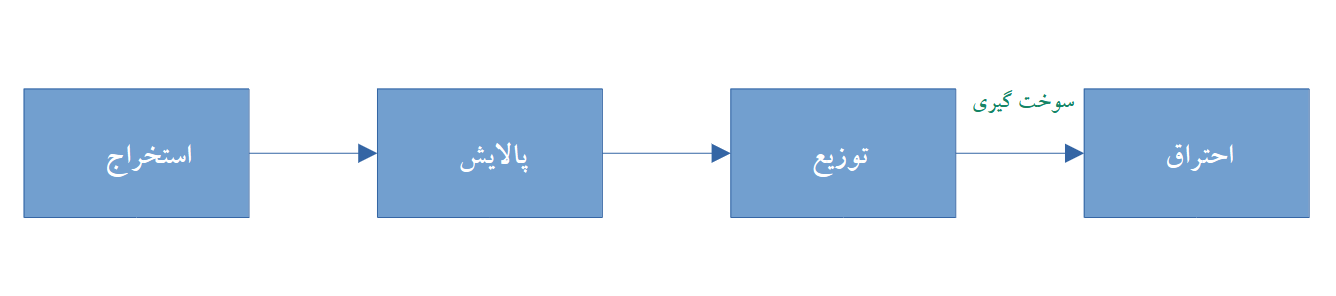
\includegraphics[width=15cm]{Figures/LPG/supply-chain.png}
 	\caption{ زنجیره تأمین سوخت}\label{Suplly-Chain}
 \end{figure}
 
\subsection{تجارت جهانی}
 تقاضای جهانی  
 \lr{LPG }
 در
  \cref{future}
 و تجارت دریایی مرتبط با آن در حال افزایش است. در سال 2022،
  تقاضای جهانی
   \lr{LPG}
    با رشد 
    $\%$5.3
    به رکورد 342 میلیون تن رسید. پیش‌بینی‌ها نشان می‌دهد که حجم تجارت دریایی
    \lr{LPG}
     در سال 2023 حدود 6 میلیون تن افزایش یافته و نسبت به 2022 رشد 5$\%$
   
      داشته است. همچنین، برای سال 2024، رشد
      $\%$3.2
        پیش‌بینی شده و انتظار می‌رود حجم تجارت تا سال 2027 به حدود 142 میلیون تن برسد.
 \begin{figure}[!h]
	\centering
	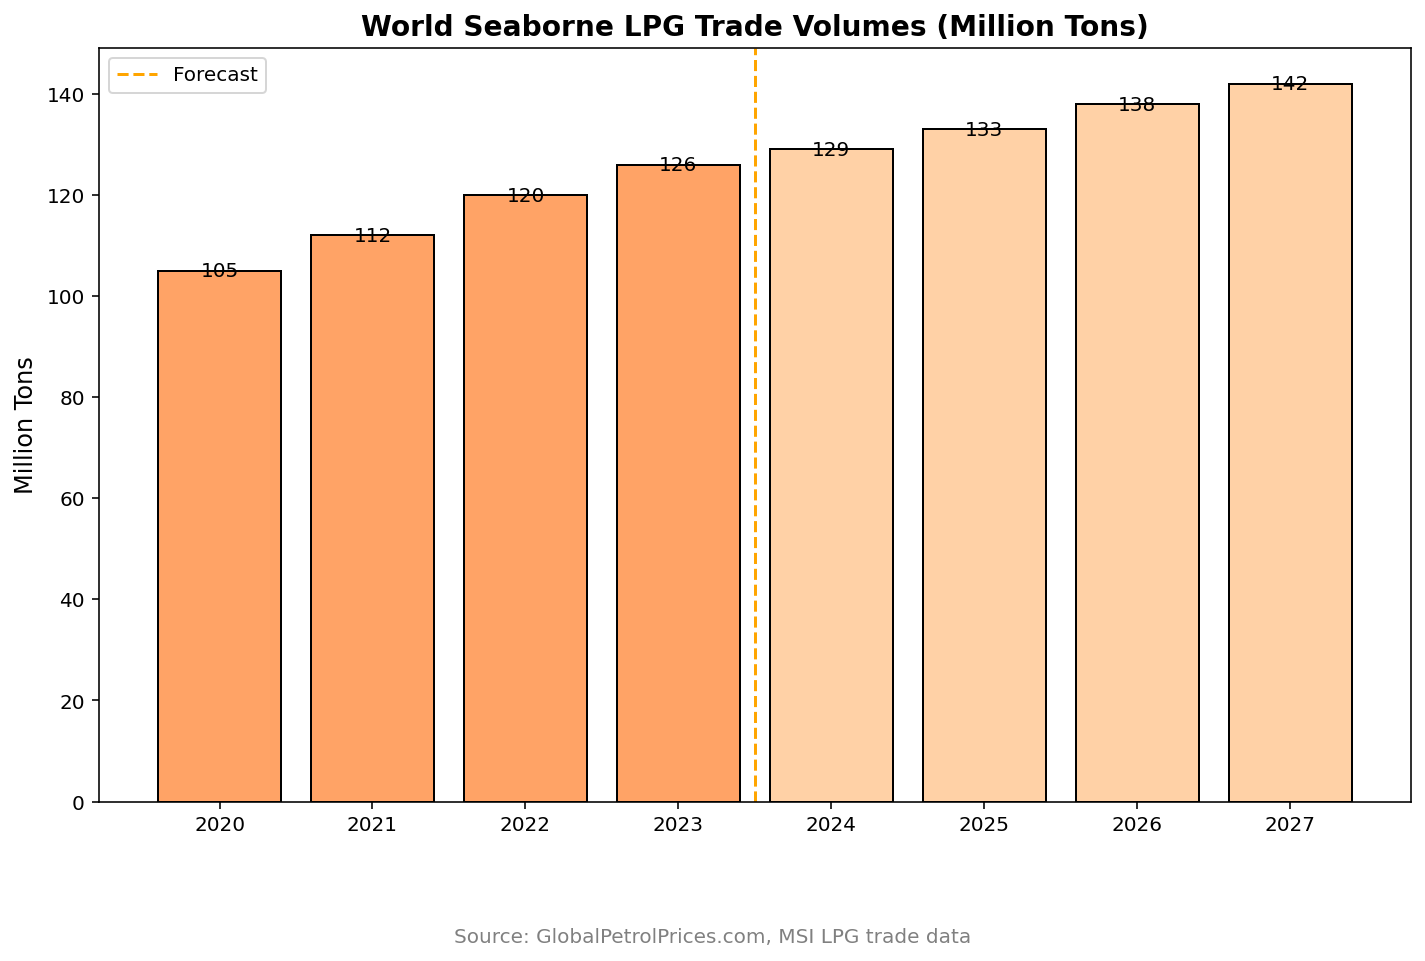
\includegraphics[width=15cm]{Figures/LPG/future.png}
	\caption{ درخواست \lr{LPG}}\label{future}
\end{figure} 
 
\subsection{قیمت سوخت}
استفاده از
 \lr{LPG}
 (گاز مایع) به عنوان سوخت، به‌دلیل قیمت جذاب آن در برخی مناطق مانند ایالات متحده و خلیج فارس، گزینه‌ای اقتصادی برای مالکان و اپراتورها محسوب می‌شود. از نظر هزینه‌های سرمایه‌ای 
 \LTRfootnote{(CAPEX)}،
  \lr{LPG }
 مزایای قابل توجهی نسبت به سایر گزینه‌های سوخت دوگانه 
\LTRfootnote{Dual-Fuel}
  مانند 
  \lr{LNG}
   دارد؛ به‌طوری که ساخت یک کشتی کانتینری ۱۰ هزار 
   \lr{TEU}
   با سوخت 
   \lr{LPG}
    حدود ۱۰۰ میلیون دلار هزینه دارد، یعنی ۲۰$\%$ ارزان‌تر از کشتی مشابه با سوخت 
    \lr{LNG }
    که حدود ۱۲۵ میلیون دلار هزینه می‌برد. همچنین، هزینه تبدیل موتورهای دیزلی به موتورهای دوگانه 
    \lr{LPG }
    (بین ۹.۵ تا ۲۷ میلیون دلار) در مقایسه با تبدیل به
     \lr{LNG}
     (بین ۱۲ تا ۳۳ میلیون دلار) مقرون‌به‌صرفه‌تر است. این عوامل باعث می‌شود.
      \lr{LPG }
      به‌عنوان گزینه‌ای جذاب برای صنعت کشتیرانی مطرح شود.
(\cref{price})
\begin{figure}[!h]
   	\centering
   		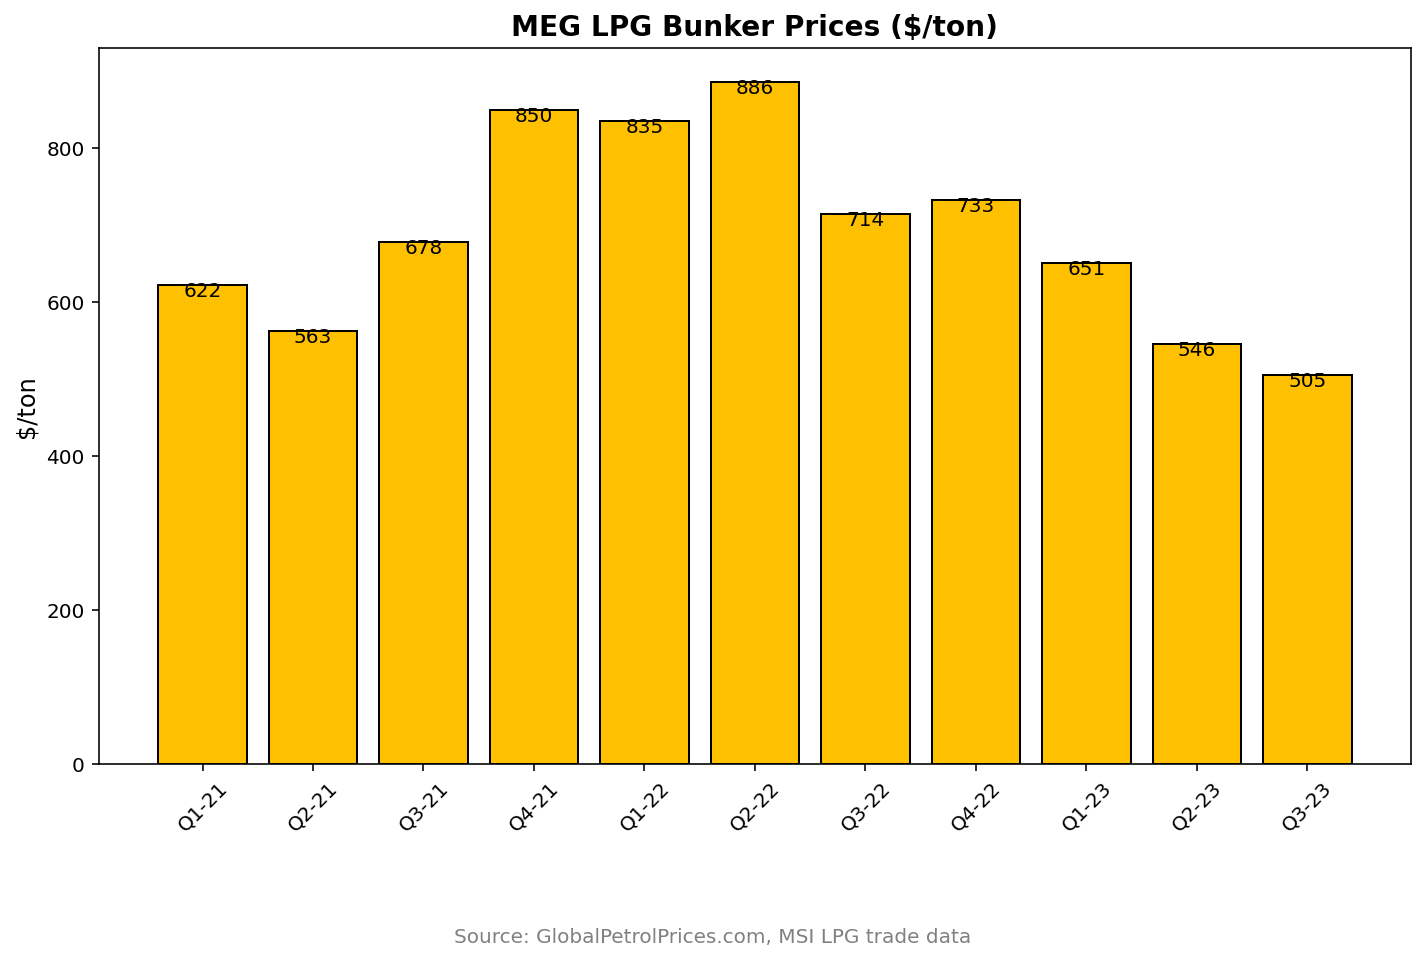
\includegraphics[width=15cm]{Figures/LPG/price.png}
   	\caption{ قیمت سوخت در خلیج فارس}\label{price}
\end{figure}
\\
\\
\subsection{تأمین و نگهداری}
\section{نتیجه‌گیری}
\begin{itemize}
	\item \textbf{مزایای زیست‌محیطی \lr{LPG}:}
	\begin{itemize}
		\item LPG به‌عنوان یک سوخت فسیلی مزیت‌های قابل توجهی در کاهش \textbf{آلودگی هوا} نسبت به سوخت‌های نفتی سنتی (مانند مازوت) دارد.
		\item استفاده از LPG موجب \textbf{کاهش انتشار گازهای گلخانه‌ای} می‌شود، به‌ویژه اگر با فناوری‌های مکملی مانند \textbf{کربن‌گیری در کشتی} همراه شود.
		\item این سوخت می‌تواند با \textbf{مقررات سازمان بین‌المللی دریانوردی (IMO)} درباره کاهش اکسیدهای گوگرد مطابقت داشته باشد و همچنین در بلندمدت با اهداف کربن‌زدایی این سازمان همخوانی داشته باشد.
	\end{itemize}
	
	\item \textbf{پتانسیل LPG برای آینده:}
	\begin{itemize}
		\item استفاده از LPG در بلندمدت به تولید سوخت‌های تجدیدپذیر وابسته است، که انتظار می‌رود با سرعت بالایی افزایش یابد.
		\item با رشد تجارت دریایی و افزایش تقاضا برای LPG، ناوگان جهانی کشتی‌های حمل LPG رشد خواهد کرد و این فرصت برای استفاده از LPG به‌عنوان سوخت افزایش می‌یابد.
		\item زیرساخت‌های حمل‌ونقل، ذخیره‌سازی و استفاده از LPG طی چند دهه به‌خوبی توسعه یافته است.
	\end{itemize}
	
	\item \textbf{چالش‌های موجود:}
	\begin{itemize}
		\item تکنولوژی‌های موتوری برای LPG محدود است. به‌عنوان مثال، هنوز موتور دریایی چهارزمانه‌ای که بتواند از LPG استفاده کند، وجود ندارد، بنابراین موتورهای کمکی کشتی‌ها نیاز به سوخت‌های دیگری برای کربن‌زدایی دارند.
		\item قوانین و چارچوب‌های مقرراتی برای استفاده از LPG به‌عنوان سوخت، خصوصاً در حوزه \textbf{سوخت‌رسانی (bunkering)}، هنوز کامل نیست و فقط راهنماهای اولیه در سطح IMO تدوین شده است.
	\end{itemize}

	\item \textbf{عامل تعیین‌کننده:}
	\begin{itemize}
		\item آینده LPG به‌عنوان یک سوخت مهم در صنعت دریانوردی به سرعت \textbf{کربن‌زدایی تولید LPG} و پیشرفت فناوری‌های مرتبط مانند \textbf{کربن‌گیری} وابسته است.
		\item همچنین LPG ممکن است به‌عنوان یک سوخت \textbf{انتقالی} تا زمان توسعه کامل سوخت‌های بدون کربن یا نزدیک به صفر کربن عمل کند.
	\end{itemize}
\end{itemize}



\chapter{مقررات و استانداردها}

\chapter{مشخصات یک پایان نامه و گزارش علمی}

اگرچه براي همه انواع نوشته‌ها، مشخصات و ويژگي‌هاي واحد و معيني نمي‌توان ذكر كرد، با اين حال در یک پایان نامه یا گزارش علمی باید نکات و موارد کلی که در این فصل ذکر می‌شود، بطور کامل رعایت شده باشد. 

دقت كنيد كه پس از عنوان فصل بايد حداقل توضیحی کوتاه در مورد موضوع نوشته شود و نمي‌توان مستقيماً بعد از آن عنوان بخش را نوشت و همين طور پس از عناوين بخش‌ها و زيربخش‌ها.(مانند دستورالعمل حاضر)
\section{برخورداری از غنای علمی }

يك پایان نامه بايد پیش از هر چيز به‌لحاظ علمي از غناي لازم برخوردار باشد. يعني هدف و پيام روشني داشته باشد و از پيش‌زمينه علمي، بيان دلايل علمی، ارجاعات مورد نیاز و نتيجه‌گيري شفاف بهره ببرد. 

\section{ارجاع به‌موقع و صحیح به منابع دیگر}
هر جمله‌ای که در یک پایان نامه نوشته می‌شود یا یک جمله کاملاً بدیهی است یا باید دلیل آن بیان شود و یا اینکه باید به منبعی که آن موضوع را نقل یا اثبات کرده، ارجاع داده شود. اگر مطلب يا گفتاري از منبعی عيناً در گزارش نقل مي‌شود، بايد آن مطلب داخل گيومه قرار گيرد و با ذكر ماخذ و شماره صفحه، به آن اشاره گردد.


\section{ساده‌نویسی }
سادگی از ضروريات يك نوشته است. نويسنده بايد ساده، روان و در عين حال شيوا و رسا بنويسد و عبارات مبهم، جملات پيچيده و كلمات نامأنوس در نوشته خود به‌كار نبرد. اگر چه افراط در اين امر نيز، به شيوايي نوشته صدمه مي‌زند. به‌كارگیری لغات و اصطلاحات دشوار و دور از ذهن و عبارات و جملات نامنظم و مبهم موجب ايجاد اشكال در فهم خواننده خواهد شد‌. 

 براي ساده‌نويسي بايد در حد امكان از به‌كارگيری كلمات «مي‌بايست»، «بايستي»، «گرديد»، «بوده باشد» و مانند آنها كه تكلف‌آور، غلط مصطلح و يا غيرشيوا هستند، به‌جای «بايد»، «است»، «شد» و مثل آنها، اجتناب شود‌.‌ همين‌طور، «در‌جهت» نمی‌تواند جايگزين خوبی برای كلمه روانی مثل «برای» باشد‌. ‌كلمات و جملات روان و ساده مي‌توانند اغلب مفاهيم را براحتی منتقل كنند‌.‌
 
دقت در تنظیم بندها (پاراگراف‌ها) نيز كمك شاياني به روانی و سادگی فهم مطلب مي‌كند‌.‌ بندهای طولانی نيز مانند جملات طولانی مي‌توانند خسته‌كننده باشند و خواننده را سردرگم كنند‌.‌ يك بند نبايد کمتر از سه یا چهار سطر یا بيشتر از $10$ تا 15 سطر باشد.‌ 

\section{وحدت موضوع}

نویسنده بايد در سراسر نوشته از اصل موضوع دور نيافتد و تمام بحث‌ها، مثال‌ها و اجزاي نوشته با هماهنگي كامل، پيرامون موضوع اصلي باشد و تاثيري واحد در ذهن خواننده القا كند. 
\section{اختصار}

پایان نامه یا گزارش علمی بايد در حد امكان، مختصر و مفيد باشد و از بحث‌هاي غير ضروري در آن پرهيز شود. نوشتن مطالب ارزشمندي كه هيچ ربطي به موضوع ندارد، فاقد ارزش علمي است.
\section{رعایت نكات دستوري و نشانه‌گذاري}
در سراسر پایان نامه بايد قواعد دستوري رعايت شود و اركان و اجزاي جمله در جاي مناسب خود آورده شود. همچنین رعايت قواعد نشانه‌گذاري سبب مي‌شود كه بيان نويسنده روشن باشد و خواننده به سهولت و با کمترین صرف انرژی مطالب را مطالعه و درك كند.
\section{توجه به معلومات ذهنی مخاطب}
نويسنده بايد همواره مخاطب خود را در برابر خود تصور كند و با توجه به معلومات ذهني مخاطب  تمامي پیش‌نیازهای لازم براي درك مطالب مورد بحث را، از پیش براي مخاطب فراهم كند.

\section{رعایت مراحل اصولی نگارش}
هر کار علمی زمانی به بهترین شکل قابل انجام است که بر اساس یک برنامه‌ریزی مشخص انجام شود. تهیه یک متن علمي با کیفیت نیز نیازمند برنامه‌ریزی مناسب و اجرای منظم آن می‌باشد. مراحل نگارش را عموماً می‌توان به ترتیب زیر درنظر گرفت:
\begin{itemize}


\item	تهيه فهرستی از عناوین اصلي و فرعی که باید نوشته شود
\item 	اولویت‌بندی و تعیین ترتیب منطقی فصل‌ها و بخش‌های گزارش
\item 	گردآوري اطلاعات اولیه راجع به هر بخش و زیربخش
\item 	تدوین مطالب جدیدی که باید به قلم نگارنده به گزارش اضافه شود
\item 	تایپ كردن مطالب با رعایت کامل نکاتی که در این دستورالعمل آموزش داده می‌شود
\end{itemize}
رعایت نظم و ترتیب در اجرای مراحل ذکر شده هم فرآیند تهیه پایان نامه یا گزارش علمی را برای نگارنده آسان می‌کند و هم کیفیت نگارش را به میزان قابل توجهی افزایش می‌دهد.

















\chapter{پیشینه تحقیق}
\usetikzlibrary{shapes.geometric, arrows}

\tikzstyle{startstop} = [rectangle, rounded corners, minimum width=3cm, minimum height=1cm,text centered, draw=black, fill=red!30]
\tikzstyle{process} = [rectangle, minimum width=3cm, minimum height=1cm, text centered, draw=black, fill=orange!30]
\tikzstyle{arrow} = [thick,->,>=stealth]


	
	\begin{tikzpicture}[node distance=2cm]
		
		\node (Covert) [startstop] {Covert};
		\node (Channel) [process, below of=Covert] {Channel};
		\node (Linguistic) [process, below of=Channel] {Linguistic};
		\node (Steganography) [process, below of=Linguistic] {Steganography};
		\node (Technical) [process, right of=Steganography, xshift=4cm] {Technical};
		\node (Information) [process, below of=Steganography] {Information};
		\node (Hiding) [process, below of=Information] {Hiding};
		\node (Anonymity) [process, below of=Hiding] {Anonymity};
		\node (Copyright) [process, below of=Anonymity] {Copyright};
		\node (Marking) [process, below of=Copyright] {Marking};
		
		\draw [arrow] (Covert) -- (Channel);
		\draw [arrow] (Channel) -- (Linguistic);
		\draw [arrow] (Linguistic) -- (Steganography);
		\draw [arrow] (Steganography) -- (Information);
		\draw [arrow] (Information) -- (Hiding);
		\draw [arrow] (Hiding) -- (Anonymity);
		\draw [arrow] (Anonymity) -- (Copyright);
		\draw [arrow] (Copyright) -- (Marking);
		\draw [arrow] (Steganography) -- (Technical);
		
	\end{tikzpicture}


%--------------------------------------------------------------------------appendix( مراجع و پیوست ها)
\chapterfont{\vspace*{-2em}\centering\LARGE}%

\appendix
\bibliographystyle{plain-fa}
\bibliography{references}
\chapter*{‌پیوست}
\markboth{پیوست}{}
\addcontentsline{toc}{chapter}{پیوست}
موضوعات مرتبط با متن گزارش پایان نامه كه در يكی از گروه‌های زير قرار می‌گيرد، در بخش پيوست‌ها آورده شوند:
\begin{enumerate}
\item  اثبات های رياضی يا عمليات رياضی طولانی‌.‌
\item داده و اطلاعات نمونه (های) مورد مطالعه (\lr{Case Study}) چنانچه طولانی باشد‌.‌
\item نتايج كارهای ديگران چنانچه نياز به تفصيل باشد‌.‌
\item مجموعه تعاريف متغيرها و پارامترها، چنانچه طولانی بوده و در متن به انجام نرسيده باشد‌.‌
\end{enumerate}
% براي شماره‌گذاري روابط، جداول و اشكال موجود در پيوست‌ از ساختار متفاوتي نسبت به متن اصلي استفاده مي‌شود كه در زير به‌عنوان نمونه نمايش داده شده‌است. 
% \begin{equation}
%F=ma
%\end{equation}
\section*{کد میپل }
\begin{latin}
\begin{verbatim}

with(DifferentialGeometry):
with(Tensor):
DGsetup([x, y, z], M)
																	frame name: M
a := evalDG(D_x)
																	D_x
b := evalDG(-2 y z D_x+2 x D_y/z^3-D_z/z^2)


\end{verbatim}
\end{latin}
%--------------------------------------------------------------------------dictionary(واژه نامه ها)
%اگر مایل به داشتن صفحه واژه‌نامه نیستید، خط زیر را غیر فعال کنید.
\parindent=0pt
%
\chapter*{واژه‌نامه‌ی فارسی به انگلیسی}
\pagestyle{style9}

\addcontentsline{toc}{chapter}{واژه‌نامه‌ی فارسی به انگلیسی}
%%%%%%
\begin{multicols*}{2}

{\bf آ}
\vspace*{3mm}


\farsiTOenglish{اسکالر}{Scalar}


\vspace*{3mm}
{\bf ب}
\vspace*{3mm}

\farsiTOenglish{بالابر}{Lift}


\vspace*{3mm}
{\bf پ}
%%\vspace*{3mm}

\farsiTOenglish{پایا}{Invariant}



\vspace*{3mm}
{\bf ت}
%%\vspace*{3mm}

\farsiTOenglish{ تناظر }{Correspondence}


\vspace*{3mm}
{\bf ث}
%%\vspace*{3mm}

\farsiTOenglish{ثابت‌ساز}{Stabilizer}

\vspace*{3mm}
{\bf ج}
%%\vspace*{3mm}

\farsiTOenglish{جایگشت}{Permutation}



\vspace*{3mm}
{\bf چ}
%%\vspace*{3mm}


\farsiTOenglish{چند جمله‌ای }{Polynomial}

\vspace*{3mm}
{\bf ح}
%%\vspace*{3mm}

\farsiTOenglish{حاصل‌ضرب دکارتی}{Cartesian product}


\vspace*{3mm}
{\bf خ}
%%\vspace*{3mm}

\farsiTOenglish{خودریختی}{Automorphism}

\vspace*{3mm}
{\bf د}
%%\vspace*{3mm}

\farsiTOenglish{درجه}{Degree}


\vspace*{3mm}
{\bf ر}
%%\vspace*{3mm}


\farsiTOenglish{ریزپردازنده}{microprocessor}


\vspace*{3mm}
{\bf ز}
%%\vspace*{3mm}


\farsiTOenglish{زیرمدول}{Submodule}


\vspace*{3mm}
{\bf س}
%%\vspace*{3mm}

\farsiTOenglish{سرشت}{Character}


\vspace*{3mm}
{\bf ص}
%%\vspace*{3mm}

\farsiTOenglish{صادقانه}{Faithful}

\vspace*{3mm}
{\bf ض}
%%\vspace*{3mm}

\farsiTOenglish{ضرب داخلی}{Inner product}

\vspace*{3mm}
{\bf ط}
%%\vspace*{3mm}


\farsiTOenglish{طوقه}{Loop}


\vspace*{3mm}
{\bf ظ}
%%\vspace*{3mm}


\farsiTOenglish{ظرفیت}{Valency}
 
\vspace*{3mm}
{\bf ع}
%%\vspace*{3mm}


\farsiTOenglish{عدم مجاورت}{Nonadjacency}



\vspace*{3mm}
{\bf ف}
%%\vspace*{3mm}

\farsiTOenglish{فضای برداری}{Vector space}



\vspace*{3mm}
{\bf ک}
%%\vspace*{3mm}

\farsiTOenglish{کاملاً تحویل‌پذیر}{Complete reducibility}


\vspace*{3mm}
{\bf گ}
%%\vspace*{3mm}


\farsiTOenglish{گراف}{Graph}



\vspace*{3mm}
{\bf م}
%%\vspace*{3mm}

\farsiTOenglish{ماتریس جایگشتی}{Permutation matrix }


\vspace*{3mm}
{\bf ن}
%%\vspace*{3mm}

\farsiTOenglish{ناهمبند}{Disconnected}


\vspace*{3mm}
{\bf و}
%%\vspace*{3mm}

\farsiTOenglish{وارون‌پذیر}{Invertible}


\vspace*{3mm}
{\bf ه}
%%\vspace*{3mm}

\farsiTOenglish{همبند}{Connected}



\vspace*{3mm}
{\bf ی}
%%\vspace*{3mm}

\farsiTOenglish{یال}{Edge}




\end{multicols*}%
%%%%%%
\chapter*{ واژه‌نامه‌ی انگلیسی به فارسی}
\pagestyle{style9}
\lhead{\thepage}\rhead{واژه‌نامه‌ی انگلیسی به فارسی}
\addcontentsline{toc}{chapter}{واژه‌نامه‌ی انگلیسی به فارسی}

\LTRmulticolcolumns
\begin{multicols}{2}
{\hfill\bf  \lr{A}}
%%\vspace*{1.5mm}

\englishTOfarsi{Automorphism}{خودریختی}

\vspace*{3mm}
{\hfill\bf   \lr{B}}
%%\vspace*{1.5mm}

\englishTOfarsi{Bijection}{دوسویی}

\vspace*{3mm}
{\hfill\bf   \lr{C}}
%%\vspace*{1.5mm}

\englishTOfarsi{Cycle group}{گروه دوری}

\vspace*{3mm}
{\hfill\bf   \lr{D}}
%%\vspace*{1.5mm}

\englishTOfarsi{Degree}{درجه}

\vspace*{3mm}
{\hfill\bf   \lr{E}}
%%\vspace*{1.5mm}

\englishTOfarsi{Edge}{یال}

\vspace*{3mm}
{\hfill\bf   \lr{F}}
%%\vspace*{1.5mm}

\englishTOfarsi{Function}{تابع}

\vspace*{3mm}
{\hfill\bf   \lr{G}}
%%\vspace*{1.5mm}

\englishTOfarsi{Group}{گروه}

\vspace*{3mm}
{\hfill\bf   \lr{H}}
%%\vspace*{1.5mm}

\englishTOfarsi{Homomorphism}{همریختی}

\vspace*{3mm}
{\hfill\bf   \lr{I}}
%%\vspace*{1.5mm}

\englishTOfarsi{Invariant}{پایا}

\vspace*{3mm}
{\hfill\bf   \lr{L}}
%%\vspace*{1.5mm}

\englishTOfarsi{Lift}{بالابر}

\vspace*{3mm}
{\hfill\bf   \lr{M}}
%%\vspace*{1.5mm}

\englishTOfarsi{Module}{مدول}

\vspace*{3mm}
{\hfill\bf   \lr{N}}
%%\vspace*{1.5mm}

\englishTOfarsi{Natural map}{نگاشت طبیعی}

\vspace*{3mm}
{\hfill\bf   \lr{O}}
%%\vspace*{1.5mm}

\englishTOfarsi{One to One}{یک به یک}

\vspace*{3mm}
{\hfill\bf   \lr{P}}
%%\vspace*{1.5mm}

\englishTOfarsi{Permutation group}{گروه جایگشتی}

\vspace*{3mm}
{\hfill\bf   \lr{Q}}
%%\vspace*{1.5mm}

\englishTOfarsi{Quotient graph}{گراف خارج‌قسمتی}

 \vspace*{3mm}
{\hfill\bf   \lr{R}}
%%\vspace*{1.5mm}

\englishTOfarsi{Reducible}{تحویل پذیر}

\vspace*{3mm}
{\hfill\bf   \lr{S}}
%%\vspace*{1.5mm}

\englishTOfarsi{Sequence}{دنباله}

 \vspace*{3mm}
{\hfill\bf   \lr{T}}
%%\vspace*{1.5mm}

\englishTOfarsi{Trivial character}{سرشت بدیهی}

\vspace*{3mm}
{\hfill\bf   \lr{U}}
%%\vspace*{1.5mm}

\englishTOfarsi{Unique}{منحصربفرد}

\vspace*{3mm}
{\hfill\bf   \lr{V}}
%%\vspace*{1.5mm}

\englishTOfarsi{Vector space}{فضای برداری}
\end{multicols}
%--------------------------------------------------------------------------index(نمایه)
%اگر مایل به داشتن صفحه نمایه نیستید، خط زیر را غیر فعال کنید.


\end{document}